%%%%%%%%%%%%%%%
% Parent document for the book Reproducible Research with R and RStudio
% Christopher Gandrud
% Updated: 31 August 2012
%%%%%%%%%%%%%%
% !Rnw weave = knitr


\documentclass[ChapterTOCs,krantz1]{krantz}\usepackage{graphicx, color}
%% maxwidth is the original width if it is less than linewidth
%% otherwise use linewidth (to make sure the graphics do not exceed the margin)
\makeatletter
\def\maxwidth{ %
  \ifdim\Gin@nat@width>\linewidth
    \linewidth
  \else
    \Gin@nat@width
  \fi
}
\makeatother

\IfFileExists{upquote.sty}{\usepackage{upquote}}{}
\definecolor{fgcolor}{rgb}{0.2, 0.2, 0.2}
\newcommand{\hlnumber}[1]{\textcolor[rgb]{0,0,0}{#1}}%
\newcommand{\hlfunctioncall}[1]{\textcolor[rgb]{0.501960784313725,0,0.329411764705882}{\textbf{#1}}}%
\newcommand{\hlstring}[1]{\textcolor[rgb]{0.6,0.6,1}{#1}}%
\newcommand{\hlkeyword}[1]{\textcolor[rgb]{0,0,0}{\textbf{#1}}}%
\newcommand{\hlargument}[1]{\textcolor[rgb]{0.690196078431373,0.250980392156863,0.0196078431372549}{#1}}%
\newcommand{\hlcomment}[1]{\textcolor[rgb]{0.180392156862745,0.6,0.341176470588235}{#1}}%
\newcommand{\hlroxygencomment}[1]{\textcolor[rgb]{0.43921568627451,0.47843137254902,0.701960784313725}{#1}}%
\newcommand{\hlformalargs}[1]{\textcolor[rgb]{0.690196078431373,0.250980392156863,0.0196078431372549}{#1}}%
\newcommand{\hleqformalargs}[1]{\textcolor[rgb]{0.690196078431373,0.250980392156863,0.0196078431372549}{#1}}%
\newcommand{\hlassignement}[1]{\textcolor[rgb]{0,0,0}{\textbf{#1}}}%
\newcommand{\hlpackage}[1]{\textcolor[rgb]{0.588235294117647,0.709803921568627,0.145098039215686}{#1}}%
\newcommand{\hlslot}[1]{\textit{#1}}%
\newcommand{\hlsymbol}[1]{\textcolor[rgb]{0,0,0}{#1}}%
\newcommand{\hlprompt}[1]{\textcolor[rgb]{0.2,0.2,0.2}{#1}}%

\usepackage{framed}
\makeatletter
\newenvironment{kframe}{%
 \def\at@end@of@kframe{}%
 \ifinner\ifhmode%
  \def\at@end@of@kframe{\end{minipage}}%
  \begin{minipage}{\columnwidth}%
 \fi\fi%
 \def\FrameCommand##1{\hskip\@totalleftmargin \hskip-\fboxsep
 \colorbox{shadecolor}{##1}\hskip-\fboxsep
     % There is no \\@totalrightmargin, so:
     \hskip-\linewidth \hskip-\@totalleftmargin \hskip\columnwidth}%
 \MakeFramed {\advance\hsize-\width
   \@totalleftmargin\z@ \linewidth\hsize
   \@setminipage}}%
 {\par\unskip\endMakeFramed%
 \at@end@of@kframe}
\makeatother

\definecolor{shadecolor}{rgb}{.97, .97, .97}
\definecolor{messagecolor}{rgb}{0, 0, 0}
\definecolor{warningcolor}{rgb}{1, 0, 1}
\definecolor{errorcolor}{rgb}{1, 0, 0}
\newenvironment{knitrout}{}{} % an empty environment to be redefined in TeX

\usepackage{alltt}
\usepackage{amssymb}
\usepackage{amsmath}
\usepackage{graphicx}
\usepackage{subfigure}
%\usepackage{epsfig}
\usepackage{makeidx}
%\usepackage{showidx}
\usepackage{multicol}
\frenchspacing
\tolerance=5000

\usepackage{dcolumn}
\usepackage{booktabs}
\usepackage{multirow}
\usepackage{pdflscape}
\usepackage{url}
\usepackage{todonotes}
\usepackage{tikz}
\usetikzlibrary{trees}




\makeatletter


\makeatother

\makeindex

\begin{document}



\title{Reproducible Research with R and RStudio}

\author{Christopher Gandrud}

\maketitle

\frontmatter

{\chapter*{Author}}

\contributor{Christopher Gandrud}{Yonsei University}{Wonju, Republic of Korea}




\chapter*{Forward}

This book would not have been possible without the advice and support of a great many people.

The developer and blogging community has been incredibly important for making this book possible. Foremost among among these people is Yihui Xie. He is the developer of the {\emph{knitr}} package (among others) and also an avid writer and reader of blogs. Without him the ability to do reproducible research would be much harder and the blogging community that spreads knowledge about how to do these things would be poorer. Other great bloggers include Carl Boettiger (who also developed the {\emph{knitcitations}} package), Markus Gesmann (who developed {\emph{GoogleVis}}), Jeromy Anglim.

The vibrant and very helpful community at Stack Overflow \url{http://stackoverflow.com/} is always very helpful for finding answers to small problems that plague any coder. Importantly it makes it easy for others to find these answers.



\chapter*{Preface}

FILL IN


\chapter*{Stylistic Conventions}\label{StylisticConventions}
\begin{noindent}




I use the following conventions throughout this book to format computer
code and actions:

\begin{itemize}
\item
  \textbf{Abstract Variables}
\end{itemize}
Abstract variables, i.e.~variables that do not represent specific
objects in an example, are in \texttt{ALL CAPS TYPWRITER TEXT}.

\begin{itemize}
\item
  \textbf{Clickable Buttons}
\end{itemize}
Clickable Buttons are in \texttt{typewriter text}.

\begin{itemize}
\item
  \textbf{Code}
\end{itemize}
All code is in \texttt{typewriter text}.

\begin{itemize}
\item
  \textbf{Filenames and Directories}
\end{itemize}
Filenames and directories more generally are printed in \emph{italics}.
Camelback is used for file and directory names.

\begin{itemize}
\item
  \textbf{Individual variable values}
\end{itemize}
Individual variable values mentioned in the text are in \textbf{bold}.

\begin{itemize}
\item
  \textbf{Objects}
\end{itemize}
Objects are printed in \emph{italics}. Camelback (e.g.~CamelBack) is
used for object names.

\begin{itemize}
\item
  \textbf{Columns}
\end{itemize}
Columns are printed in \emph{italics}

\begin{itemize}
\item
  \textbf{Packages}
\end{itemize}
\textbf{R} packages are printed in \emph{italics}.

\begin{itemize}
\item
  \textbf{Windows}
\end{itemize}
Open windows are written in \textbf{bold} text.

\begin{itemize}
\item
  \textbf{Variable Names}
\end{itemize}
Variable names are printed in \emph{italics}. Camelback is used for
individual variable names.





\chapter*{Required R Packages}\label{ReqPackages}

This book discusses how to use a number of user-written R packages for reproducible research. These are not included in the default R installation (see Section \ref{InstallR}). They need to be installed installed separately. To install all of the user-written packages discussed in this book use the following code:

\begin{knitrout}
\definecolor{shadecolor}{rgb}{0.969, 0.969, 0.969}\color{fgcolor}\begin{kframe}
\begin{alltt}
\hlfunctioncall{install.packages}(\hlstring{"apsrtable"}, 
                \hlstring{"devtools"}, 
                \hlstring{"ggplot2"}, 
                \hlstring{"knitr"}, 
                \hlstring{"knitcitations"}, 
                \hlstring{"markdown"}, 
                \hlstring{"openair"}, 
                \hlstring{"texreg"},                     
                \hlstring{"xtable"}, 
                \hlstring{"Zelig"})
\end{alltt}
\end{kframe}
\end{knitrout}






\end{noindent}

\listoffigures
\listoftables
\tableofcontents

\mainmatter

\setcounter{page}{1}

\part{Getting Started}

% Chapter Chapter 1 For Reproducible Research in R and RStudio
% Christopher Gandrud
% Created: 16/07/2012 05:45:03 pm CEST
% Updated: 29 August 2012




\chapter{Introducing Reproducible Research}\label{Intro}

Most people encounter research as a neat and very abridged package. This package is usually in the form of a conference presentation, journal article, book, or maybe even a website. These presentation documents announce the results of some research project and try to convince us that the results are correct.\cite{Mesirov2010}. However, the article, slideshow, or book is not the research. 
\section{What is reproducible research?}

FILL IN

\section{Why should research be reproducible?}

Incorporating high reproducibility into your research is important for science and it can also make your life as a researcher easier. 

\subsection{For Science}

\subsection{For You}

Working to make your research reproducible from the start has a number of knock on benefits that make the research process easier {\emph{for the researcher}}. A third person may or may not actually reproduce your research even if you make it easy to do so. But, it's almost certain that you will reproduce parts or even all of your research. Virtually no actual research process is completely linear. We almost never gather data, run our analyses, and present our results without also going backwards to add variables, make changes to our statistical models, create new graphs, and so on. Whether these changes are because of journal reviewers' and conference participants comments or we discover that new and better data has been made available since beginning the project, designing our research to be reproducible from the start makes it much easier to make these changes. 

Changes made to one part of a research project have a way of cascading through the other parts. For example, adding a new variable to a largely completed analysis requires gathering new data and merging it into existing data sets. If we are using data imputation or matching methods this can lead to adjustments to the entire data set. We then have to update our statistical models and the tables and graphs we use to present results. Adding a new variable essentially forces us to reproduce large portions of our research. If we made it easier for others do reproduce our research we also made it easier for us to do this. Jake Bowers has referred to this as taking steps to have a ``better relationship with our future selves".\cite{Bowers2011}

COMPLETE

\section{Who should read this book?}

This book is intended primarily for upper-level undergraduate and graduate students and professional researchers who want to develop a more systematic workflow that encourages reproducibility.

\subsection{Students}

\subsection{Researchers}

\subsection{Industry practitioners}

Industry practitioners may or may not want to make their work easily reproducible outside of their organization. However, that does not mean that significant benefits cannot be gained from using the methods of reproducible research. First, even if public reproducibility is ruled out to guard proprietary information, making your research reproducible to members of your organization can save and pass on valuable information about how analyses were done and data collected. Just as a lack of reproducibility hinders the spread of information in the scientific community, it can hinder it inside of a private organization. COMPLETE

\section{The Tools of Reproducible Research}

This book will teach you the tools you need to make your research highly reproducible. Reproducible (quantitative) research involves two broad sets of tools. The first is a {\bf{reproducible research environment}} that includes the statistical tools you need to run your analyses as well as ``the ability to automatically track the provenance of data, analyses, and results and to package them (or pointers to persistant versions of them) for redistribution". The second set of tools is a {\bf{reproducible research publisher}} that prepares documents to present the results and is easily linked to the reproducible research environment.\cite{Mesirov2010}

In this book I we will focus on learning how to use widely available and highly flexible reproducible research environment--R/RStudio. R/RStudio can be linked to numerous reproducible research publishers with Yihui Xie's {\emph{knitr}} package\cite{knitr}. The full list of tools tools covered in this book include:

\begin{itemize}
    \item {\bf{R}}: a programming language primarily for statistics and graphics. It can also be used for data gathering and creating presentation documents.
    
    \item {\bf{{\emph{knitr}}}}: an R package for literate programming\index{literate programming}, i.e. it allows us to combine our statistical analysis and the presentation of the results into one document.
    
    \item {\bf{Markup languages}}: instructions for how to format a presentation document. In this book we cover \LaTeX and Markdown.  
    
    \item {\bf{RStudio}}: an integrated developer environment (IDE)\index{integrated developer environment} for R that tightly integrates R, {\emph{knitr}}, and markup languages.
    
    \item {\bf{Cloud storage \& versioning}}: Services such as Dropbox and Github that can store research, save and document previous versions, and make this information widely available.
    
    \item {\bf{Unix-like shell programs}}: These tools are useful for setting up and working with large research projects.\footnote{In this book I cover the Bash shell for Linux and Mac as well as Windows PowerShell.} They also allow us to use command line tools like Pandoc for converting documents from one markup language to another.
\end{itemize}

\section{Why use R/RStudio for reproducible research?}

\paragraph{Why R?}
Why use a statistical programming language like R for reproducible research? R is more than just a statistics program, like \index{SAS}, Stata\index{Stata}, or SPSS\index{SPSS}. It can be used to integrate all stages of the research process not just the statistical analysis stage. As we will see in this book, R can be used to gather data, run statistical analyses, and we can use the {\emph{knitr}} R package to connect our analysis to our presentation documents created with markup languages\index{markup language} such as \LaTeX, Markdown, and HTML we can dynamically present our results in articles, slideshows, and webpages.\footnote{When we use these types of markup languages to create presentation documents what we write is text plus the instructions for how to turn this into a final document. The instructions are written using a markup language. Part IV of this book (Presentation Documents) discusses how to use the \LaTeX and Markdown languages for reproducible research.} 

The way we interact with R or any other programming and markup language promotes reproducibility more than our interactions with Graphical User Interface (GUI) programs like SPSS\footnote{I know you can write scripts in statistical programs like SPSS, but doing so is not encouraged by the interface and we often have to learn multiple languages just to write scripts that run analyses, create graphics, and deal with matrices.} and Microsoft Word. When we write (and save) R code and embed it in documents using markup languages we are being forced to explicitly express the steps we take to do our research. When we do research clicking through drop down menus in GUI programs, the steps we take are lost. Or at least documenting them requires considerable extra effort.

\paragraph{Why RStudio?}
\index{RStudio}Why use the RStudio integrated development environment for reproducible research? R by itself has the capability to gather data, analyse it, and with a little help from {\emph{knitr}} and markup languages, present results in a way that is highly reproducible. RStudio allows us to do all of these things, but simplifies many of these tasks and allows you to navigate them in a more visual way. It is a as happy medium between R's text-based interface and a pure GUI. 

{\emph{RStudio is designed for reproducible research}}. RStudio is very tightly integrated with technologies such as {\tt{knitr}}, Markdown, and \LaTeX that enable us to present reproducible results. Compiling \LaTeX PDF documents or HTML webpages in RStudio requires many fewer steps than doing the same thing in plain R. 

Not only does RStudio do many of the things that R can do, but more easily it is very good stand alone editor for writing documents with \LaTeX, Markdown, HTML. There are many \LaTeX editors available, both open source and paid, as well as other ways to compile \LaTeX documents, including directly through the command line. RStudio is currently the best program for creating reproducible \LaTeX, Markdown, and HTML documents. It has full syntax highlighting, even for documents with \texttt{knitr} code (which it can collapse when you just
want to work on the text). It can spell check \LaTeX documents. It handles \texttt{knitr} code chunks beautifully making it easy to navigate through complex documents and run individual chunks. For \LaTeX documents it can, for example, insert common commands like \texttt{\textbackslash{}section*\{\}} for unnumbered sections or set up lists. 

Finally, RStudio not only has tight integration with various markup languages, it also integrates other tools such as CSS, JavaScript, and a few other programming languages as well as being closely integrated with the version control programs git and SVN. Both of these programs allow you to keep track of the changes you make to your documents. This is important for reproducible research since the version control program is documenting many of the the steps you took to make your project. As with many tools of reproducible research, version control has other benefits for making researchers' lives easier. Maybe most importantly, when you keep your documents under version control you can go back to older versions. This is useful if you accidentally delete an important paragraph, for example.

\subsection{Installing the Software}\label{InstallR}

Before you read this book you should install the software. All of the software covered in detail in this book is open source programs and can be easily downloaded for free. It is available for Windows\index{Windows}, Mac\index{Mac}, and Unix\index{Unix}. They should run well on most modern computers. 

You should install R before installing RStudio. You can down load the programs from the following websites:

\begin{itemize}
    \item {\bf{R}}: \url{http://www.r-project.org/},
    \item {\bf{RStudio}}: \url{http://rstudio.org/download/}.
\end{itemize}

\noindent The download webpages for these programs have comprehensive information on how to install them, so please refer to those pages for more information.

After installing R and RStudio you will probably want to additionally install a number of user-written packages that are covered in this book. To install all of these user-written packages, please see the \ref{ReqPackages}.

\paragraph{Installing markup languages}

If you are planning on creating \LaTeX documents you need to install a \LaTeX distribution\index{\LaTeX distribution}. They are also open source and available for Windows, Mac, and Unix. They can be found at: \url{http://www.latex-project.org/ftp.html}. Please refer to that site for more installation information.

If you want to create markdown documents you will need to install the the \index{{\emph{markdown}} package} in R. You can do this the same way that you install any package in R, with the {\tt{install.packages}} command.\footnote{The exact command is: {\tt{install.packages("markdown")}}.} 

\paragraph{The command line}

\paragraph{Cloud storage \& versioning}

\section{Book overview}

The purpose of this book is to give you the tools that you will need to do reproducible research with R and RStudio. 

\subsection{What this book is not.}\label{WhatNot}

This book describes a workflow for reproducible research primarily using R and RStudio. It is designed to give you the necessary tools to use this workflow for your own research. It is not designed to be a complete introduction to R, RStudio, GitHub, the command line, or any other program that is a part of this workflow. Instead it shows you how these tools can fit together to make yourß research more reproducible.

To get the most out of these individual programs I point you to other resources that cover these programs in more detail.

That being said, my goal in this for this book to be self-sufficient to the extent that a reader without a detailed understanding of these programs will be able to understand and use the commands and procedures
I cover in this book. While learning how to use R and the other programs I often encountered examples that included commands, variables, and other things that were not well explained in the texts that I was reading. This caused me to waste many hours trying to figure out, for example, what the \texttt{\$} is used for (preview: it's the `component selector'). I hope to save you from this wasted time by either providing a brief explanation of
these possibly frustratingly mysterious conventions and/or pointing you in the direction of a good explanation.

To that end, I can recommend a number of books for that cover more of the nitty-gritty of R and the command line.

\begin{itemize}
    \item Michael J. Crawley's encyclopaedic R book, appropriately   titled, \textbf{The R Book} published by Wiley.
    
    \item Norman Matloff's tour through the programming language aspects of  R called \textbf{The Art of R Programming: A Tour of Statistical Design Software} published by No Starch Press.
    
    \item For an excellent introduction to the command line in Linux and Mac, though with pretty clear implications for Windows users if they are running PowerShell (see Chapter 2) see William E. Shotts Jr.'s book \textbf{The Linux Command Line: A Complete Introduction} also published by No Starch Press.
    
    \item The RStudio website (\url{http://rstudio.org/docs/}) has a
  number of useful tutorials on how to use {\emph{knitr}} with \LaTeX and Markdown.
\end{itemize}

\subsection{How to read this book.}

This book tells a story. It has a beginning, middle, and end. So, unlike a reference book it can and should be read like a novel, taking you through an empirical research processes from an empty folder maybe called {\emph{ResearchPaper}} to a completed set of documents that showcase your findings.

That being said, readers with more experience using tools like R or \LaTeX) may want to skip over the nitty-gritty parts of the book that describe how to manipulate data frames or compile a \LaTeX) document into a PDF. Please feel free to do this.

If you are experienced with R in particular you may want to skip over the first two sections of Chapter \ref{GettingStarted}: Getting Started with R/RStudio. The latter part of this chapter contains important basic information on the {\emph{knitr}} package. 

\subsection{How this book was written}

This book practices what it preaches. It can be reproduced. It was written using the programs and methods that it describes. Full documentation and source files can be found at the Book's \textbf{GitHub} repository. Feel free to read and even copy (within reason and with attribution, of course) the Book's source code. You can find it at \url{https://github.com/christophergandrud/Rep-Res-Book}. This is especially useful if you want to know how to do something in the book that I don't directly cover in the text.

In the same spirit, I encourage you to make your research files--not just data, but analysis code and markup--available for other researchers to learn from. Not only does reproducibility help us evaluate past work, but it also pushes forward knowledge in the scientific community.

\subsection{Contents overview.}

% Chapter Chapter 2 For Reproducible Research in R and RStudio
% Christopher Gandrud
% Created: 16/07/2012 05:45:03 pm CEST
% Updated: 29 August 2012




\chapter{Getting Started with Reproducible Research}\label{GettingStarted}

Researchers often start thinking about making their research reproducible near the end of the research process when they get start writing up the results. Or maybe later, like when a journal has conditioned an article's acceptance on making its data available or another researcher asks if they can use the data. By this point there may be various versions of the data set and records of the analyses strewn across multiple folders on the researcher's computer. It can be difficult and time consuming to create an accurate account of how the results were reached. As a result many attempts at providing replication information are incomplete and may not give us an accurate account of how research results were found. Keeping your eye on reproducibility from the beginning of the research process and continuing to follow a few simple guidelines throughout your research can help solve these problems. 

This chapter first gives you a big picture overview of the reproducible research process: a workflow for reproducible research. Then it covers some of the key guidelines that can help make your research more reproducible.

\section{The Big Picture: A workflow for reproducible research}

To make our research accurately reproducible we should start thinking at the beginning--the data gathering stage--about how other researchers and ourselves will be able to reproduce our results. This book teaches the tools for an integrated workflow for reproducible research. It covers tools that we can use across the three basic stages that most researchers--especially quantitative researchers--go through to answer their research questions:

\begin{itemize}
    \item data gathering,
    \item data analysis,
    \item results presentation.
\end{itemize}

\subsection{Data Gathering}

It is common in many disciplines (I know this is true in political science, my discipline) to 

\subsection{Data Analysis}

\subsection{Results Presentation}

\section{Practical tips for reproducible research}

Before we start learning the details of reproducible research with R and RStudio it is useful to cover a few broad tips that will help us organize our research process and put these skills in perspective. The tips are:

\begin{enumerate}
    \item Document everything!,
    \item Everything is a file,
    \item All files should be human readable,
    \item Reproducible research projects are many files explicitly tied together,
    \item Have a plan to organize, store, and make your files available.
    
\end{enumerate}

\subsection{Document everything!}

In order to reproduce your research others must be able to know what you did. You have to tell them what you did by documenting as much of your research process as possible. Ideally, you should tell your readers how you gathered your data, analyzed it, and presented the results.

The other tips and Many of the other One important part of documenting everything with R is to \emph{record your session info\index{session info}}. Many things in R stay the same over time, which makes it easy for future researchers to recreate what was done in the past. However, things--syntax in particular--do can change from one version of R to another. Also, the way R functions may be handled slightly different on different operating systems. Finally, you may have R set to load packages by default. These packages might be necessary to run your code, but other people might not be able know what packages were loaded from just looking at your source code. The \texttt{sessionInfo} command prints a record of all of these things. The information from the session I used to create this book up until this chapter is:

\begin{knitrout}
\definecolor{shadecolor}{rgb}{0.969, 0.969, 0.969}\color{fgcolor}\begin{kframe}
\begin{alltt}
\hlfunctioncall{sessionInfo}()
\end{alltt}
\begin{verbatim}
## R version 2.15.1 (2012-06-22)
## Platform: x86_64-apple-darwin9.8.0/x86_64 (64-bit)
## 
## locale:
## [1] C/en_US.UTF-8/C/C/C/C
## 
## attached base packages:
## [1] stats     graphics  grDevices utils     datasets 
## [6] methods   base     
## 
## other attached packages:
## [1] knitcitations_0.1-0 bibtex_0.3-0       
## [3] knitr_0.7.9        
## 
## loaded via a namespace (and not attached):
##  [1] RCurl_1.91-1    XML_3.9-4       codetools_0.2-8
##  [4] digest_0.5.2    evaluate_0.4.2  formatR_0.6    
##  [7] pkgmaker_0.8    plyr_1.7.1      stringr_0.6.1  
## [10] tools_2.15.1    xtable_1.7-0
\end{verbatim}
\end{kframe}
\end{knitrout}


\noindent It is good practice to include make output of the session info available either in the main document or in a separate text file. If you want to nicely format the information for a \LaTeX document simply use the {\tt{toLatex}} command.

\begin{knitrout}
\definecolor{shadecolor}{rgb}{0.969, 0.969, 0.969}\color{fgcolor}\begin{kframe}
\begin{alltt}
\hlfunctioncall{toLatex}(\hlfunctioncall{sessionInfo}())
\end{alltt}
\end{kframe}
\end{knitrout}


\noindent Otherwise, you can use the {\tt{print}} command. 

\subsection{Everything is a (text) file}

Your documentation is stored in files that include data, analysis code, the write up of results, and explanations of these files (e.g. data set codebooks, session info files, and so on). Ideally, you should use the simplest file format possible to store this information. Usually the simplest file format is the the humble, but versatile, text file is the simplest file format.\footnote{Depending on the size of your data set it may not be feasible to store it as a text file. Nonetheless, text files can still be used for analysis code and presentation files.} 

Text files are extremely nimble. They can hold data in, for example, comma-separated values {\tt{.csv}} \index{comma-separated values6} files. They can contain our analysis code in {\tt{.R}} files. And they can be the basis for our presentation documents as markup documents like {\tt{.tex}} or {\tt{.md}}, for \LaTeX and Markdown files respectively. All of these files can be opened by any program that can read text files--i.e. files with the generic file extension {\tt{.txt}}. 

The main reason reproducible research is best stored in text files is that this helps {\bf{future proof}} our research. Other common file formats, like Microsoft Word \index{Microsoft Word} or Excel \index{Microsoft Excel} documents change regularly and may not be compatible with future versions of these programs. Text files, on the other hand, can be opened by a very wide range past and, more likely than not, future programs. Even if future researchers do not have R or a \LaTeX distribution, they will still be able to open our text files and, aided by frequent comments, be able to understand how we conducted our research.

Text files are also very easy to search and manipulate with a wide range of programs--such as R--that can find and replace text characters as well as merge and separate files. They have a number of clear benefits for reproducible research including enabling versioning and track changes in programs such as Git (see Chapter \ref{Storing}).   

\subsection{All files should be human readable}

Treat all of your research files as if someone who has not worked on the project will try to read them and understand them. Computer code is a way of communicating with the computer. It is `machine readable' in that the computer is able to use it to understand what we want done.\footnote{Of course, if it does not understand it will usually give us an error message.} Hopefully, the researcher understands what they are communicating when they write their code. However, there is a very good chance that other people (or the researcher six months in the future) will not understand what is being communicated. So, you need to make your documentation `human readable'. To make your documentation accessible to other people you need to {\bf{comment frequently}} and {\bf{format your code using a style guide}}. For especially important piece of code you should use {\bf{literate programming}} so that it is very clear to others how you accomplished a piece of research.

\paragraph{Commenting}
In R everything on a line after a {\tt{\#}} hash (number) character is ignored by R, but is readable to people who open the file. The hash character is a comment declaration\index{comment declaration} character. You can use the {\tt{\#}} to place comments telling other people what you are doing. Here are some examples:

\begin{knitrout}
\definecolor{shadecolor}{rgb}{0.969, 0.969, 0.969}\color{fgcolor}\begin{kframe}
\begin{alltt}
\hlcomment{# A complete comment line}
2 + 2  \hlcomment{# A comment after R code}
\end{alltt}
\begin{verbatim}
## [1] 4
\end{verbatim}
\end{kframe}
\end{knitrout}


Because on the first line the {\tt{\#}} is placed at the very beginning, the entire line is treated as a comment. On the second line the {\tt{\#}} is placed after the simple equation {\tt{2 + 2}}. R runs the equation as usual and fines the answer {\tt{4}}, but it ignores all of the words after the hash. 

Different languages have different comment declaration characters. In \LaTeX everything after the {\tt{\%}} percent sign is treated as a comment and in markdown/HTML comments are placed inside of {\tt{\textless !-- --\textgreater}}. The hash character is used for comment declaration in shell scripts.

\paragraph{Style guides}
In natural language writing you don't necessarily need to follow a \index{style guide} for things such as punctuation. People could probably figure out what you are saying. But it would be a lot easier for your readers if you use consistent rules. The same is true when writing R code. It's good to follow consistent rules for formatting your code so that:

\begin{itemize}
    \item it's easier for others to understand,
    \item it's easier for you to understand.
\end{itemize}

There are a number of R style guides. Most of them are similar to the Google R Style Guide \index{Google R Style Guide} (\url{http://google-styleguide.googlecode.com/svn/trunk/google-r-style.html}). Hadley Wickham \index{Hadley Wickham} has a nicely presented style guide. You can find it at \url{https://github.com/hadley/devtools/wiki/Style}. You can also use the {\tt{formatR}} \index{\tt{formatR}} package to automatically reformat your code so that it is easier to read.

\paragraph{Literate programming}

For particularly important pieces of research code it may be useful to not only comment on the source file, but also display code in presentation text. For example, you may want to include key parts of the code you used for your statistical model and an explanation of this code in an appendix following your article. This is commonly referred to as literate programming \index{literate programming} \cite{Knuth1992}. This book discusses how to use the {\emph{knitr}} package, a very useful tool for literate programming. 

\subsection{Reproducible research projects are many files explicitly tied together}

If everything is just a text file then research projects can be thought of as individual text files that have a relationship with one another. A data file is used as input for an analysis file. The results of an analysis are shown and discussed in a markup file that is used to create a slideshow or PDF document. Researchers often do not explicitly document the relationships between files that they used in their research. For example, the results of an analysis--a table or figure--may be copied and pasted into a presentation document. It will be very difficult for future researchers to trace the results table or figure back to a particular analysis and a particular data set. Therefore, it is important to make the links between your files explicit. 

The most dynamic way to do this is to explicitly link your files together using what I'll call {\bf{tie commands}}. \index{tie commands} These commands instruct the computer program you are using to gather data, run an analysis, or compile a presentation document to use information from another file. I have compiled the main tie commands used in this book in Table \ref{TableTieCommands}.

\begin{landscape}
\begin{table}
    \caption{Commands for Tying Together Your Research Files}
    \label{TableTieCommands}
    \vspace{0.3cm}
    \begin{tabular}{l c  p{6.5cm}  m{4cm}}
        \hline
        Command/Package & Language & Description & Chapters for Further Information \\  
        \hline \hline
        {\emph{knitr}} & R & R package with functions for tying R commands into presentation documents & Discussed throughout the book \\
        {\tt{read.table}} & R & Reads a table into R & \ref{DataGather} \\
        {\tt{source}} & R & Runs an R source code file & \ref{StatsModel} \\
        {\tt{source\_url}} & R & From the {\emph{devtools}} package. Runs an R source code file from a secure ({\tt{https}}) url like those used by GitHub & \ref{StatsModel} \\
        {\tt{input}} & \LaTeX & Includes \LaTeX files inside of other \LaTeX files & \ref{LargeDocs} \\
        {\tt{include}} & \LaTeX & Similar to {\tt{input}}, but puts page breaks on either side of the included text. Usually this it is used for including chapters chapters. & \ref{LargeDocs} \\
        
        \hline 
        
    \end{tabular}
\end{table}
\end{landscape}


\subsection{Have a plan to organize, store, and make your files available}

% Chapter Chapter 3 For Reproducible Research in R and RStudio
% Christopher Gandrud
% Created: 16/07/2012 05:45:03 pm CEST
% Updated: 3 September 2012




\chapter{Getting Started with R, RStudio, and knitr}\label{GettingStarted}

If you have rarely or never used R before the first two sections of this chapter give you enough information to be able to get started and understand the code I use in this book. For more detailed introductions to R please refer to the related resources I mentioned in chapter \ref{WhatNot}. Experienced R users might want to skip the first two sections of the chapter. This chapter also gives a brief overview of RStudio. It highlights the key features of main RStudio panel (what appears when you open RStudio) and some of its key features for reproducible research. Finally, I discuss the basics of the {\emph{knitr}} package and how it is integrated into RStudio.

%%%%%%%%%%%%% Using R
\section{Using R: the basics}

As a computer language, R has FILL in

This section covers some of the very basic syntax in R to get you started. If you have little experience with R, reading this section will make it much easier for you to follow along with the examples in the book. I cover the key components of the R language including:

\begin{itemize}
    \item objects \& assignment,
    \item component selection,
    \item functions, commands, and arguments,
    \item libraries.
\end{itemize}

Before discussing each of these components let's open up R and look around.\footnote{Please see Chapter \ref{Intro} for instructions on how to install R.} When you open up R you should get a window that looks something like what you see in Figure \ref{RBlankMain}.\footnote{This figure and almost all screenshots in this book are from a computer using the Mac OS 10.8 operating system.} This window is the {\bf{R console}}\index{R console}. Under the session\index{session information} information--what version of R you are using, your workspace, and so on--you should see a {\tt{\textgreater}}. This is where you enter R code.\footnote{If you are using a Unix-like system such as Ubuntu or Mac OS 10, you can an application called the Terminal\index{Terminal}. If you have installed R on your computer you can type {\tt{r}} into the terminal and then the {\tt{Enter}} or {\tt{Return}} key it will begin a new R session. You know if a new R session has started if you get the same startup information is printed in the Terminal window.} To run R code that you have typed into the console type the {\tt{Enter}} or {\tt{Return}} key. Now that we have a new R session open we can get started. 

\begin{figure}[th!]
    \caption{R Startup Console}
    \label{RBlankMain}
    \begin{center}
    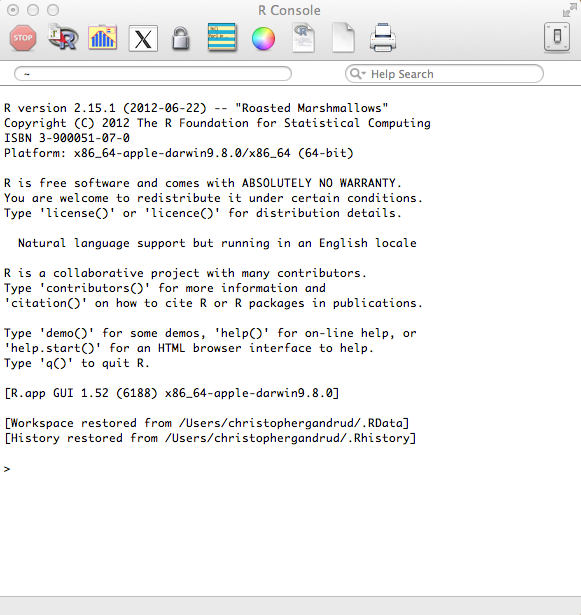
\includegraphics[scale=0.4]{/git_repositories/Rep-Res-Book/Source/Children/Chapter3/images3/BlankRConsole.png}
    \end{center}
\end{figure}

\subsection{Objects}

You will probably have read that `R is an object-oriented\index{object-oriented} language'.  What are objects? Objects are like the R language's nouns. They are things, such as a list of numbers, a data set, a word, a table of results from some analysis, and so on. Saying that R is `object-oriented' just means that R is focused on doing actions to objects. We will talk about the actions--commands and functions--later in this section. For now let's create a few objects.

\paragraph{Numeric \& string objects}

Different types of objects have different classes\index{object classes}. Let's make two basic objects of the numeric and character classes. We can choose almost any name we want for our objects.\footnote{Objects must begin with an alphabetic character and cannot have spaces.} Let's call our numeric object {\emph{Number}}. To put something into the object we use the {\bf{assignment operator}}: {\tt{\textless -}}. Let's assign the number 10 to our Number object.

\begin{knitrout}
\definecolor{shadecolor}{rgb}{0.969, 0.969, 0.969}\color{fgcolor}\begin{kframe}
\begin{alltt}
Number <- 10
\end{alltt}
\end{kframe}
\end{knitrout}


\noindent To see the contents of our object, just type its name.

\begin{knitrout}
\definecolor{shadecolor}{rgb}{0.969, 0.969, 0.969}\color{fgcolor}\begin{kframe}
\begin{alltt}
Number
\end{alltt}
\begin{verbatim}
## [1] 10
\end{verbatim}
\end{kframe}
\end{knitrout}


\noindent \texttt{10} is clearly the contents of {\emph{Number}}. The double has \texttt{\#\#} is included in the output by {\emph{knitr}} to tell you that this is output rather than R code.\footnote{This makes it easier to copy and past code included in a presentation document by {\emph{knitr}}.} Finally, \texttt{[1]} is the row number of the object that 10 is on. Clearly our object only has one row.   

Creating a character object is very similar. The only difference is that we enclose the character string (letters in a word for example) inside of quotation marks ({\tt{""}}). To create an object called {\emph{Words}} that contains a character string ``Hello World".

\begin{knitrout}
\definecolor{shadecolor}{rgb}{0.969, 0.969, 0.969}\color{fgcolor}\begin{kframe}
\begin{alltt}
Words <- \hlstring{"Hello World"}
\end{alltt}
\end{kframe}
\end{knitrout}



An object's class is important to keep in mind as it determines what things we can do to it. For example you cannot take the mean of a character class object like the {\emph{Words}} object we created earlier:

\begin{knitrout}
\definecolor{shadecolor}{rgb}{0.969, 0.969, 0.969}\color{fgcolor}\begin{kframe}
\begin{alltt}
\hlfunctioncall{mean}(Words)
\end{alltt}


{\ttfamily\noindent\textcolor{warningcolor}{\#\# Warning: argument is not numeric or logical: returning NA}}\begin{verbatim}
## [1] NA
\end{verbatim}
\end{kframe}
\end{knitrout}


\noindent Trying to find the mean of our {\emph{Words}} object gave us a warning message and returned the value {\tt{NA}}\index{NA}: not applicable. You can also think of {\tt{NA}} to mean missing. To find out what class an object has use the {\tt{class}} command. For example:

\begin{knitrout}
\definecolor{shadecolor}{rgb}{0.969, 0.969, 0.969}\color{fgcolor}\begin{kframe}
\begin{alltt}
\hlfunctioncall{class}(Words)
\end{alltt}
\begin{verbatim}
## [1] "character"
\end{verbatim}
\end{kframe}
\end{knitrout}


\paragraph{Vector \& data frame Objects}

Sp far we have only looked at objects with a single number or string.\footnote{These might be called scalar objects, though in R scalars are just vectors with a length of 1.} Clearly we want to be using objects--data sets--that have many strings and numbers. In R these are usually {\bf{data frame}}\index{data frame} type objects and are roughly equivalent to the type of data structure you would be familiar with from using a program such as Microsoft Excel. We will be using data frames extensively throughout the book. It is also useful to cover other, simpler types of objects, primarily vectors. Vectors are R's ``workhorse".\cite{Matloff2011} Knowing how to use vectors\index{vector} will be especially helpful when we clean up raw data in Chapter \ref{DataClean} and make tables in Chapter \ref{TablesChapter}.\footnote{If you want information about other types of R objects such as lists\index{list} and matrices\index{matrix}, Chapter 1 of Norman Matloff's book\cite{Matlof2011} is a really good place to look.} \\[0.25cm]

\noindent {\bf{Vectors}}: \\[0.25cm] Vectors are the ``fundamental data type"\cite{Matloff2011} in R. They are simply an ordered group of numbers, character strings, and so on.\footnote{In a vector every member of the group must be of the same type. Lists are similar to vectors, but allow you to have different types.} It may be useful to think of basically all other data types as complicated forms of vectors. For example, data frames are basically multiple vectors of the same length--i.e. they have the same number of rows--attached together. 

Let's create a very simple numeric vector containing the numbers 1, 17, 24, and 6. To do this we will use the \texttt{c} (concatenate)\index{concatenate} function:

\begin{knitrout}
\definecolor{shadecolor}{rgb}{0.969, 0.969, 0.969}\color{fgcolor}\begin{kframe}
\begin{alltt}
NumericVect <- \hlfunctioncall{c}(1, 17, 24, 6)

\hlcomment{# Show NumericVect's contents}
NumericVect
\end{alltt}
\begin{verbatim}
## [1]  1 17 24  6
\end{verbatim}
\end{kframe}
\end{knitrout}



\noindent {\bf{Data frames}}: 


\subsection{Component Selection}

Smaller objects can be combined into larger objects. For example, a data set with two variables may be merged into a larger data set. We will touch on some of these issues, like how to use the {\tt{merge}} command in Chapter \ref{DataGather}. Sometimes we may want to do the opposite task: extract a smaller object from a larger one. We can do this with the dollar sign ({\tt{\$}}). This is called the component selection\index{component selection}, because we use it to select a component from an object.

For example, 

This will be especially useful when we discuss making tables for presentation documents in Chapter \ref{TablesChapter}.

\subsection{Functions, Commands, and Arguments}

\subsection{Loading new commands from libraries}

You can install new user-written packages using the {\tt{install.packages}} command. By default this command downloads and installs the packages from the Comprehensive R Archive Network (CRAN)\index{CRAN}. To install all of the package libraries used in this book see \ref{ReqPackages}.

Commands are stored in R libraries\index{R libraries}. R automatically loads a number of basic libraries by default. One of the great things about R is the many user-created libraries\footnote{For the latest list see: \url{http://cran.r-project.org/web/packages/available_packages_by_name.html}} that greatly expand the number of commands we can use. 

%%%%%%%%%%%%%%% Using RStudio
\section{Using RStudio}

As I mentioned in Chapter \ref{Intro} When you first open RStudio\index{RStudio} you should get a something that looks like Figure \ref{BlankMain}. In this figure you see three panels\index{RStudio panels}. The large one on the left is the {\emph{Console}}. This pane functions exactly the same as the console in regular R. 

\begin{figure}[ht]
    \caption{RStudio Startup Panel}
    \label{BlankMain}
    \begin{center}
    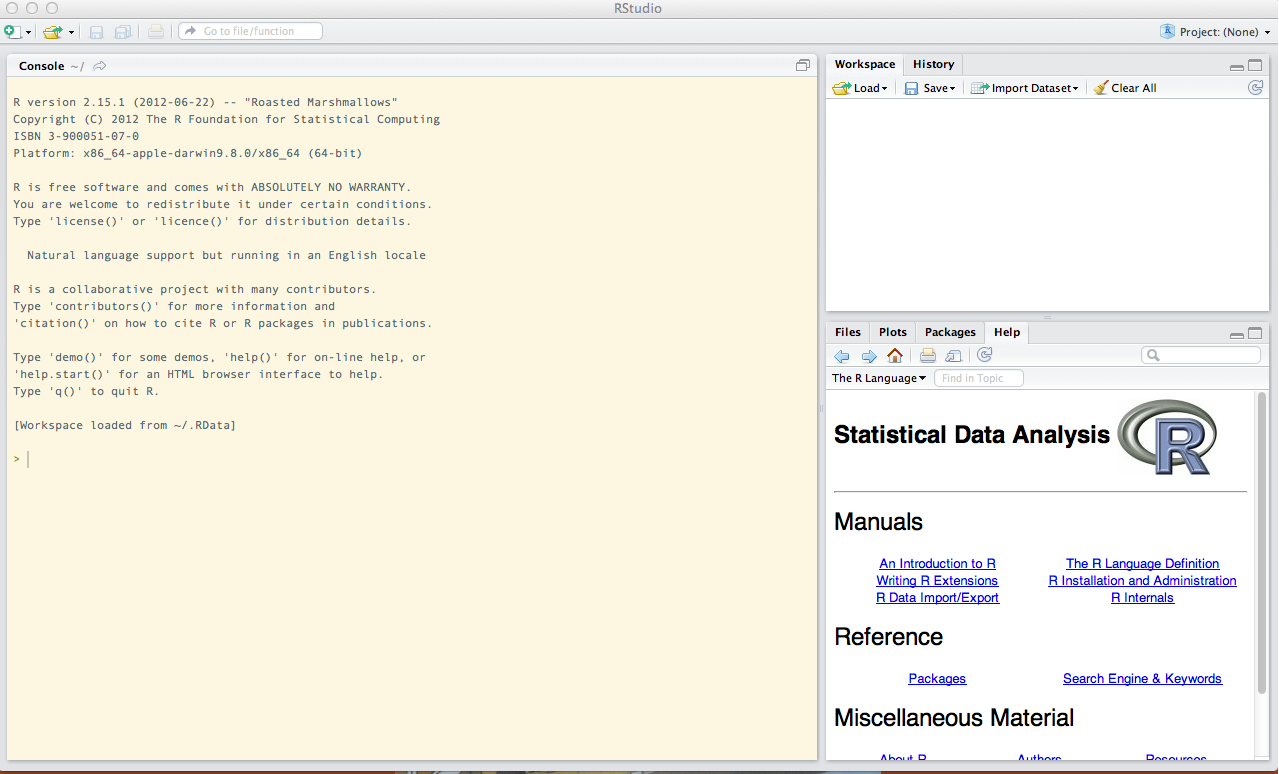
\includegraphics[width = \textwidth]{/git_repositories/Rep-Res-Book/Source/Children/Chapter3/images3/BlankMainPanel.png}
    \end{center}
\end{figure}

\paragraph{Compile Notebook}

RStudio integrates a number of different methods for literate programming. The most basic is 

%%%%%%%%%%%%% Using knitr
\section{Using knitr: the basics}

For more advanced literate programming in R we can use the {\emph{knitr}}\index{{\emph{knitr}}} package.\footnote{The RStudio notebook actually also uses {\emph{knitr}}.} This package is highly integrated into RStudio. Throughout much of the book we cover many details about how to use {\emph{knitr}}. This section gives you a basic introduction to get started.

\subsection{Code Chunks}

When we want to include R code into our presentation documents we place them in a code chunk\index{code chunk}.

FILL IN

All labels and code chunk options must be on the same line.

\paragraph{Code chunk labels}

\paragraph{Code chunk options}

For the full list of {\emph{knitr}} options see this page maintained by {\emph{knitr}}'s creator Yihui Xie: \url{http://yihui.name/knitr/options#package_options}.

\subsection{Code Chunk Options Markup Language Specific Syntax}

The code chunk options discussed so far are specifically for presentation documents written in Markdown syntax. Though the syntax for {\emph{knitr}} options is the same regardless of the markup language we use 

\paragraph{Code Chunks in Markdown}

\paragraph{Code Chunks in \LaTeX}

\LaTeX documents that include {\emph{knitr}} code chunks are generally called R Sweave\index{R Sweave} files and have the file extension {\tt{.Rnw}}. This terminology is a little confusing. It is a holdover from {\emph{knitr}}'s main literate programming predecessor {\emph{Sweave}}.\cite{Leisch2002} More recent versions of {\tt{knitr}} support files with the {\tt{.Rtex}} extension, though the code chunk syntax is different. I will cover both types of syntax for code chunks in \LaTeX documents, though in throughout the book I use the older and more established {\emph{Sweave}} style syntax. \\[0.25cm]

\noindent {\bf{.Rnw-style}} \\[0.25cm]

\noindent {\bf{.Rtex-style}} \\[0.25cm]

\subsection{Global Options}

So far we have only looked at how to set local options\index{local chunk options} in {\emph{knitr}} code chunks. If we want an option to apply to all of the chunks in our document we can set {\bf{global chunk options}}\index{global chunk options}. They options are `global' in the sense that they apply to the entire document. Setting global chunk options helps us create documents that are formatted consistently without having to repetitively specify the same option every time we create a new code chunk. For example, in this book I center almost all of the the figures. Instead of using the {\tt{fig.align='center'}} option in each code chunk that creates a figure I set the option globally.

To set a global option first create a new code chunk at the beginning of your document\footnote{In Markdown, you can put global chunk options at the very top of the document. In \LaTeX they should be after the \texttt{\textbackslash{}begin\{document\}} command (see Chapter \ref{LatexChapter} for more information on how \LaTeX documents are structured).} You will probably want to set the option {\tt{echo=FALSE}} so that {\emph{knitr}} doesn't echo the code. Inside the code chunk use {\tt{opts\_chunk\$set}}. You can set any chunk option as an argument to {\tt{opts\_chunk\$set}}. The option will be applied across your document, unless you set a different local option. 

Here is an example of how we could have all of the figures in a Markdown document created by {\emph{knitr}} code chunks center aligned. We place the following code at the beginning of the document:

\begin{knitrout}
\definecolor{shadecolor}{rgb}{0.969, 0.969, 0.969}\color{fgcolor}\begin{kframe}
\begin{alltt}
```\{r GlobalFigOpts, echo=FALSE\}
\hlcomment{# Center align all knitr figures}
opts_chunk$\hlfunctioncall{set}(fig.align=\hlstring{'center'})
```
\end{alltt}
\end{kframe}
\end{knitrout}


\subsection{knitr package options}

Chunk options determine how we want to treat code chunks. We can also set package options\index{package options} that affect how the {\emph{knitr}} package itself runs. For example, the {\tt{progress}} option can be set as either {\tt{TRUE}} or {\tt{FALSE}}\footnote{It's set as {\tt{TRUE}} by default.} depending on whether or not we want a progress bar\index{progress bar} to be displayed when we knit a code chunk.\footnote{The {\emph{knitr}} progress bar looks like this {\tt{|>>>>>>| 100\%}} and indicates how much of a code chunk has been run.} You can use {\tt{base.dir}} to set the directory where you want all of your figures to be saved to (see Chapter \ref{DirectoriesChapter}) or the {\tt{child.path}} option to specify where child documents are located (see Chapter \ref{LargeDocs}).

We set package options in a similar way to global chunk options with {\tt{opts\_knit\$set}}. For example, to turn off the progress bar when knitting Markdown documents include this code at the beginning of the document:

\begin{knitrout}
\definecolor{shadecolor}{rgb}{0.969, 0.969, 0.969}\color{fgcolor}\begin{kframe}
\begin{alltt}
```\{r GlobalFigOpts, echo=FALSE\}
\hlcomment{# Turn off knitr progress bar}
opts_knit$\hlfunctioncall{set}(progress=FALSE)
```
\end{alltt}
\end{kframe}
\end{knitrout}



\subsection{knitr \& Rstudio}

\subsection{knitr \& R}

As an R package, you can of course knit documents in regular R (or using the console in RStudio). All of the syntax in the document you are knitting is the same as before. But instead of clicking a {\tt{Compile PDF}} or {\tt{knit HTML}} button we use is {\tt{knit}} command. To knit our example Markdown file {\emph{Example.Rmd}} we first set the working directory (see Chapter \ref{DirectoriesChapter}) to the the folder where your {\emph{Example.Rmd}} file is located with the {\tt{setwd}} command. In this example I have it on my desktop.\footnote{Using the directory name {\tt{~/Desktop/}} is for Mac computers. Please use alternative syntax discussed in Chapter \ref{DirectoriesChapter} on other types of systems.}

\begin{knitrout}
\definecolor{shadecolor}{rgb}{0.969, 0.969, 0.969}\color{fgcolor}\begin{kframe}
\begin{alltt}
\hlfunctioncall{setwd}(\hlstring{"~/Desktop/"})
\end{alltt}
\end{kframe}
\end{knitrout}


\noindent Then I knit my file:

\begin{knitrout}
\definecolor{shadecolor}{rgb}{0.969, 0.969, 0.969}\color{fgcolor}\begin{kframe}
\begin{alltt}
\hlfunctioncall{knit}(input = \hlstring{"Example.Rmd"}, output = \hlstring{"Example.md"})
\end{alltt}
\end{kframe}
\end{knitrout}


\noindent Note that if you do not specify the output file {\emph{knitr}} will determine what the file should be. In this example it would come up with the same name and location.

If you try this example, you find that the {\emph{knit}} command only created a Markdown file and not an HTML file like clicking the RStudio {\tt{knit HTML}} did. Likewise, if you use {\tt{knit}} on a {\tt{.Rnw}} file you will only end up with a basic \LaTeX {\tt{.tex}} file and not a compiled PDF. To convert the Markdown file into HTML you need to further run the {\tt{.md}} file through the {\tt{markdownToHTML}} command from the {\emph{markdown}} package, i.e.

\begin{knitrout}
\definecolor{shadecolor}{rgb}{0.969, 0.969, 0.969}\color{fgcolor}\begin{kframe}
\begin{alltt}
\hlfunctioncall{mardownToHTML}(file = \hlstring{"Example.md"}, output = \hlstring{"Example.html"})
\end{alltt}
\end{kframe}
\end{knitrout}


\noindent If we want to compile a {\tt{.tex}} file in R we run it through the {\tt{texi2pdf}} command in the {\emph{tools}} package. This package will run both \LaTeX and \BibTeX to create a PDF with a bibliography (see Chapter \ref{LatexChapter} for more details on using \BibTeX for bibliographies). Here is a {\tt{texi2pdf}} example:

\begin{knitrout}
\definecolor{shadecolor}{rgb}{0.969, 0.969, 0.969}\color{fgcolor}\begin{kframe}
\begin{alltt}
\hlfunctioncall{texi2pdf}(file = \hlstring{"Example.tex"})
\end{alltt}
\end{kframe}
\end{knitrout}

 
\section{R/RStudio Tips}

Finally, here are a few other tips that make using R and RStudio a little easier.

\paragraph{Getting Help}

You can quickly access the help file for any command. In R/the Rstudio console simply type {\tt{?}} before any command. For example, to get the help file for the {\tt{mean}} command just type:

\begin{knitrout}
\definecolor{shadecolor}{rgb}{0.969, 0.969, 0.969}\color{fgcolor}\begin{kframe}
\begin{alltt}
?mean
\end{alltt}
\end{kframe}
\end{knitrout}


\noindent In RStudio you can click on the {\bf{Help}} pane (by default at the lower right, see Figure \ref{BlankMain}) and enter the command you want help with into the search field.

\paragraph{Autocomplete}

In R and RStudio you do not have to type out every command, argument, object, or even directory name. After you start typing a command/argument/object/directory name you can hit the ``tab" key to automatically complete the word you started. The \index{autocomplete} function is particularly good in RStudio. Not only does it give you a list of words to choose from, but it also shows you an abbreviated version of the help file for commands and arguments.


% Chapter Chapter 4 For Reproducible Research in R and RStudio
% Christopher Gandrud
% Created: 16/07/2012 05:45:03 pm CEST
% Updated: 2 September 2012




\chapter{Getting Started with File Management}\label{DirectoriesChapter}

Careful file management is crucial for reproducible research. Apart from the fleeting situations where you have am email exchange (or even meet in person) someone interested in reproducing your research, the main information other researchers will have is stored across many files: data files, analysis files, and presentation files. If these files are well organized then replication will be easier. File management is also important for you as a researcher, because if your files are well organized you will be able to understand your work more easily. Remember two of the guidelines from Chapter \ref{GettingStarted}:

\begin{itemize}
    \item Reproducible research projects are many files explicitly tied together,
    \item Have a plan to organize, store, and make your files available. 
\end{itemize}

Using tools such as R and markup languages like \LaTeX requires a bit more knowledge of how files are located--their {\bf{path}}\index{file path}--in your computer and on the internet than just knowing which graphical folder they are located in. Though more difficult to use at first than the typical point-and-click graphical user interface file handling systems you are probably familiar, R and Unix-like shell programs allow us to control files--creating, deleting, moving them--in powerful and reproducible ways. 

In this chapter we discuss how a reproducible research project may be organized and cover the basics of file path naming conventions\index{file path naming conventions} in Unix, Mac, and Windows systems. We then learn how to navigate through files in RStudio in the {\bf{Files}} pane as well as some basic R and Unix-like shell commands for manipulating files. The skills we learn in this chapter will be heavily used in the next Chapter (Gathering Data with R) and throughout the book.

In this chapter we work with locally stored files\index{locally stored}, i.e. files stored on your computer. In the next chapter (Chapter \ref{Storing}) we will discuss various ways to store and access files stored remotely in the cloud\index{cloud storage}.

\section{Organizing your research project}

Figure \ref{ExampleTree} gives an example of how the files in a simple reproducible research project could be structured. The project--called {\emph{Example Project}}--is organized into three main parts: a data gathering section, an analysis section, and a presentation section. The results of the project are presented in an article, slideshow, and website.

\clearpage
\thispagestyle{plain}
\begin{landscape}
\begin{figure}[th!]
    \caption{Example Research Project File Tree}
    \label{ExampleTree}
    \begin{center}
    
    \documentclass{article}

\usepackage{tikz}

\begin{document}

%%%%%% Example 

\tikzstyle{DirBox} = [draw=black, rectangle, minimum width=5em, thick]
  
\begin{tikzpicture}
  % Root Directory
  \node (root) at (5, 10) [DirBox]{Root};
  
  % Project Directory
  \node (project) at (5, 8.5) [DirBox]{Project};
  
  % Main Project sub-directories
  \node (data) at (2, 7) [DirBox]{Data};
  \node (analysis) at (5, 7) [DirBox]{Analysis};
  \node (presentation) at (8, 7) [DirBox]{Presentation};
  
  % Data subdirectories/files
  \node (dataGatherSource) at (-0.5, 6) [DirBox]{GatherSource};  
  \node (dataFiles) at (2, 6) [DirBox]{DataFiles};
  
  \node (dataMake) at (-0.5, 5.25) {{\small{DataMakeFile.R}}};
  
  \node(dataGather) at (-0.5, 4.5) [DirBox]{IndvDataGather};
  \node (dataGather1) at (-0.5, 3.5) {{\small{DataGather1.R}}};
  
  % Analysis subdirectores/files
  
  % Presentation subdirectories/files
  
  % Connect boxes
  \draw (root) -- (project);
  \draw (project) -| (data);
  \draw (project) -- (analysis);
  \draw (project) -| (presentation);
  
  %% Data connect boxes
  \draw (data) -| (dataGatherSource);
  \draw (data) -- (dataFiles);
  \draw (dataGatherSource) -- (dataMake);
  
\end{tikzpicture}



\end{document}
    \end{center}
\end{figure}
\end{landscape}

\section{File paths \& naming conventions}

All of the operating systems\index{operating systems} covered in this book use organize files in in hierarchical directories\index{directories} (or file trees). To a large extent, `directories' can be thought of as the folders you usually see on your Windows or Mac desktop. They are called `hierarchical' because directories are located inside of other directories, like we saw in Figure \ref{ExampleTree}. 

\subsection{Root directories}

\subsection{Working directories}

\section{Operating system-specific naming conventions}

\paragraph{Unix}

\paragraph{Mac}

\paragraph{Windows}

\section{File navigation in RStudio}

The RStudio {\bf{Files}} pane allows us to navigate and do some basic file manipulations. Figure \ref{FilesPane} shows us what this pane looks like.

\begin{figure}[t!]
    \caption{The RStudio Files Pane} \\[0.25cm]
    \label{FilesPane}
        \begin{center}    
        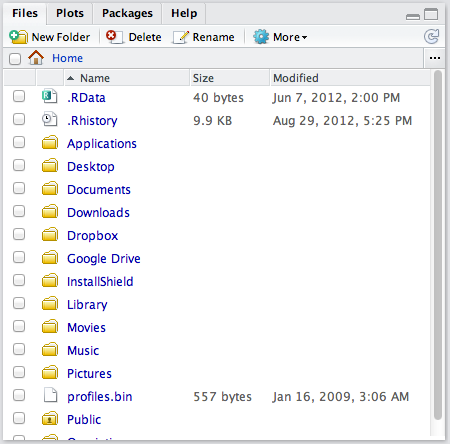
\includegraphics[scale=0.4]{/git_repositories/Rep-Res-Book/Source/Children/Chapter4/images4/RStudioFiles.png}
        \end{center}
\end{figure}

\section{R file manipulation commands}

All of the tasks we can accomplish in RStudio's {\bf{Files}} pane can also be accomplished using command line R. This allows us to more easily replicate our actions. 

\paragraph{{\tt{setwd}}}

The {\tt{setwd}} command sets the working directory.

\paragraph{{\tt{dir.create}}}

Sometimes we may want to create a new directory. We can use the {\tt{dir.create}} command to do this.

\paragraph{{\tt{unlink}}}

You can use the {\tt{unlink}} command to delete a file, files, or directories. 

\section{Unix-like shell commands} 

Though this book is mostly focused on using R for reproducible research it can be useful to use a Unix-like shell program to manipulate files in large projects. A command line shell program is simply a program that allows you to type commands to interact with your computer's operating system.\cite{ShottsJr2012} We will especially return to shell commands near the end of the book when we discuss Make files\index{Make files} for compiling large documents, and batch reports\index{batch reports} (Chapter \ref{LargeDocs}). The syntax discussed here is also similar to the used in command line git (Chapter \ref{Storing}) and Pandoc (Chapter \ref{LargeDocs}). We don't have enough space to properly get started with shell programs. For good introductions for Unix and Mac OS 10 computers see William E. Shotts Jr.'s book on the Linux command-line\cite{ShottsJr2012} and for Windows users Microsoft maintains a tutorial on Windows PowerShell at \url{http://technet.microsoft.com/en-us/library/hh848793}.

The one piece of general instruction I will give now is to highlight an important difference in the syntax between R and shell commands. In shell commands you don't need to put parentheses around your arguments. For example if we want to change our working directory to my Mac Desktop in a shell using the {\tt{cd}} command we simply type:

\begin{knitrout}
\definecolor{shadecolor}{rgb}{0.969, 0.969, 0.969}\color{fgcolor}\begin{kframe}
\begin{alltt}
cd ~/Desktop
\end{alltt}
\end{kframe}
\end{knitrout}


\paragraph{{\tt{cd}}}

As we just saw, to change the working directory in the shell can just use the {\tt{cd}}\index{cd} (change directory) command.

\paragraph{{\tt{rm}}}

The {\tt{rm}}\index{rm} command is similar to R's {\tt{unlink}} command. It deletes files or directories.


\part{Data Gathering and Storage}

% Chapter Chapter 5 For Reproducible Research in R and RStudio
% Christopher Gandrud
% Created: 16/07/2012 05:45:03 pm CEST
% Updated: 2 September 2012




\chapter{Storing, Collaborating, Accessing Files, Versioning}\label{Storing}

A stumbling block to actually reproducing a piece of research is getting a hold of the datasets and the codebooks that describe the data used in
an analysis.

Researchers often face a number of data management issues that, beyond
making their research difficult to reproduce, can make doing the initial
research difficult.

First, there is the problem of \textbf{storing} the data so that it is
protected against computer failure--virus infections, spilling coffee on
your laptop, and so on.

Fourth, we almost never create a data set or write a paper perfectly all
at once. We may make changes and then realize that we liked an earlier
version, or parts of an earlier version better. This is a particularly
important issue in data management where we may transform our data in
unintended ways and want to go back to an earlier version. Collaborative
projects can have regular incidents of one author accidentally deleting
something in a file that another author needed, for example.

To deal with these issues we need to store our data in a system that has
\textbf{version control}. Version control systems keep track of changes
we make to our files and allow us to access previous versions if we
like.

the data set can often grow and become disorganized. Perhaps even during
a data transformation This creates problems

You can solve all of these problems in a couple of different ways using
free or low cost cloud-based storage formats. In this chapter we will
learn how to use Dropbox and GitHub for data:

\begin{itemize}
    \item storage,
    \item accessing,
    \item collaboration,
    \item version control.
\end{itemize}

\section{Saving data in reproducible formats}

Before getting into the details of cloud-based data storage, lets just
consider what type of formats you should actually save your data in. A
key issue for reproducibility is that others be able to not only get
ahold of the exact data you used in your analysis, but be able to
understand and use the data not only now, but in the future. Some file
formats make this easier than others.

R is able to read (and write) a very wide variety of file
formats, mostly through the \texttt{foreign} package in \texttt{base}
R. This includes

\section{Storing data in the cloud}

Storing data locally--on your computer--or on a flash drive is generally
more prone to loss than storing data on remote servers, often referred
to as `the cloud'.

\section{Dropbox}

The easiest types of cloud storage for your research are services like
Dropbox and Google Drive. These services typically
involve a folder based on your computer's hard drive that is
automatically synced with a similar folder on a cloud-based server.
Typically you can sign up for the service for free and receive a limited
amount of storage space (usually a few gigabytes, which should be plenty
if your research is made up of text files.).

Most of these services not only store your data in the cloud, but also
provide some way to share files and maybe even includes basic version
control. I am going to focus on using Dropbox because it
currently offers a complete set of features that allow you to store,
version, collaborate, and access your data.

\subsection{Version control}

Dropbox has a simple version control system. Every time you
save a document on Dropbox a new version is created. One the
Dropbox website

\subsection{Accessing Data}

There are two similar, but importantly different ways to access data
stored on Dropbox. All files stored on Dropbox have a
URL address through which they can be access from computer connected to
the internet. Some of these files can be easily loaded directly into
R, while others must me manually (point-and-click) downloaded
onto your computer and then loaded into R. The key factor is
whether or not the files are located in your \textbf{Dropbox}'s
\emph{Public} folder. Files in the \emph{Public} folder can be
downloaded directly into R. Files not in the \emph{Public} folder
have to be downloaded manually.\footnote{This is not completely true. It
  is possible to create a web scraper (see Chapter GET) that could
  download a data file from a file not in your \emph{Public} folder.
  However, this is kind of a hassle and not practical, especially since
  the accessing files from the \emph{Public} folder is so easy.}

Either way you find a file's URL address by first right-clicking on the
file icon in you Dropbox folder. If the file is stored in the
\emph{Public} folder, you go to Dropbox then \textbf{Copy
Public Link}. This copies the URL into your clipboard from where you can
paste it into your R source code (or wherever). Once you have
the URL you can load the file directly into R using the
\texttt{read.table} command for dataframes (see Chapter 5) or the \texttt{source}
command for source files (see Chapter 8).

If the file is not in your \emph{Public} folder you also go to
Dropbox after right-clicking. Then choose \textbf{Get Link}.
This will open a webpage in your default web browser from where you can
download the file. You can copy and paste the page's URL from your
browser's address bar.

You can also get these URL links through the online version of your
Dropbox. First log into the Dropbox website. When you
hover your curser over a file (or folder) name you will see a chain icon
appear on the far right. Clicking on this icon will get you the link.

Storing files in the \emph{Public} folder clearly makes replication
easier because the files can be downloaded and run directly in
R.

Note that you cannot save files through the URL link. You must save
files in the Dropbox folder on your computer.

\section{GitHub}

Dropbox does a fine job of meeting our four basic criteria for
reproducible data storage. GitHub meets these criteria and
more.

GitHub was not explicitly designed to host research projects or
even data. It was designed to host `socially coded' computer programs.
It built an interface on top of the git version control system
that makes it easy relatively easy for a number of collaborators to work
together to build a computer program. This seems very far from
reproducible research.

However, remember that as reproducible researchers we are just building
projects out of interconnected text files. This is exactly the same as
computer programming. and like computer programers, we need ways to
store, version control, access, and collaborate on our text files.
Because GitHub is very actively used by people with very
similar needs (who are also really good programmers), the interface
offers many highly developed and robust features for reproducible
researchers.

As is usually the case, GitHub's added features mean that it is
takes a longer time than Dropbox to set up and become familiar.
So we need good reasons to want to invest the time needed to learn
GitHub rather than just sticking with Dropbox or a
similar service. Here is a list of GitHub's key features
relative to Dropbox for reproducible research:

\begin{itemize}
\item
  Git is directly integrated into RStudio projects
  (\textbf{RStudio} also supports the subversion version
  control system, but I don't cover that here).
\item
  Dropbox's version control system only lets you the see the
  file names, the times they were created, who created them, and revert
  back to specific versions. git tracks every change you make
  in a way that makes it relatively easy to find the version you want.
  The GitHub website and GUI programs for Mac and Windows
  provide nice interfaces for examining specific changes. You can also
  use the command line to see changes.
\item
  Dropbox creates a new version every time you save a file,
  which can make it difficult to actually find the version you want.
  git's version control system only creates a new version when
  you tell it to.
\item
  Dropbox does not merge conflicting versions of a file
  together. This can be annoying when you are collaborating on project
  and more than one author is making changes to documents.
  GitHub identifies conflicts and lets you reconcile them.
\item
  The GitHub website as an `'Issues'' area where you can to
  note and discuss issues you have while doing your research. Basically
  this is an interactive to-do list for your research project.
\end{itemize}

\subsection{Setting Up GitHub}

There are a number of ways to set up GitHub on your computer. I
will briefly cover both the command line version (available for Windows,
Mac, and Linux) and the GUI\footnote{Graphical User Interface, i.e.~not
  the command line version, but the one with windows that you navigate
  with your mouse.} version currently available only for Windows and
Mac.

\subsection{Version Control in GitHub}

GitHub's version control system is much more comprehensive than Dropbox's. However, it also has a steeper learning curve.

\paragraph{Reverting to an old version of a file}

You can use the {\tt{git checkout}} command to revert to a previous version of a document, because you accidentally deleted something important or made other changes you don't like. To 'checkout' a particular version of a file type:

\begin{knitrout}
\definecolor{shadecolor}{rgb}{0.969, 0.969, 0.969}\color{fgcolor}\begin{kframe}
\begin{alltt}
git checkout COMMITREF FILENAME
\end{alltt}
\end{kframe}
\end{knitrout}


\noindent Now the previous version of the file is in your working directory, where you can commit it as usual.

Let's break down the code.  {\tt{FILENAME}} is the name of the file that you want to change\footnote{If it is in a repository's subdirectory you will need to include this in the file name.} and {\tt{COMMITREF}} is the reference that git gave to the commit you want to revert back to. The reference is easy to find and copy in GitHub. On the file's GitHub page click on the {\tt{History}} button. This will show you all of the commits. By clicking on {\tt{Browse Code}} you can see what the file at that commit looks like. Above this button is another with a series of numbers and letters. This is the commit's SHA (Secure Hash Algorithm). For our purposes, it is the commit's reference number. Click on the {\tt{Copy SHA}} button to the left of the SHA to copy it. You can then paste it as an argument to your {\tt{git checkout}} command. 

\paragraph{More Practice with Command Line GitHub}

If you want more practice setting up GitHub in the command
line, GitHub and the website Code School have an interactive
tutorial that you might find interesting. You can find it at:
\url{http://try.github.com/levels/1/challenges/4}.
% Chapter Chapter 6 For Reproducible Research in R and RStudio
% Christopher Gandrud
% Created: 16/07/2012 05:45:03 pm CEST
% Updated: 2 September 2012




\chapter{Gathering Data with R}\label{DataGather}

There are many practical issues involved in gathering data that can make replication easier or harder. As with all of the steps in this book: document everything. Replication will be easier if your documentation--source code--can be understood and executed by a computer. Of course there are data gathering situations that simply require manually pointing and clicking, talking with subjects in an experiment, and so on. The best we can do in these situations is just describe our data gathering process in detail CITE. Nonetheless, R's automated data gathering capabilities are extensive and often under utilized. Learning how to take full advantage of them greatly increases replicability and can even save researchers considerable time and effort.

\section{Organize Your Data Gathering: Make files}

Before getting into the details of using R to automate data gathering, lets's start from where all data gathering should start: a plan to organize the process. Clearly organizing your data gathering process from the start of a research project improves the possibility of replicability and can save significant effort over the course of the project. 

A key principle of replicable data gathering with R, like replicable research in general is segmenting the process into discrete files that can be run by a common Make file. The Make file's output is the data set(s) that we use in the statistical analyses. There are two types of files that the Make file runs: data clean up files and merging files. Data clean up files bring raw (the rawer the better) individual data sources into R and transform them into something that can be merge with data from the other sources. Some of the R tools for data clean up were covered in Chapter 3. In this chapter we mostly cover the ways to bring raw data into R. We don't explicitly cover the process of merging data sets together in this book GET CITE. Merging files are executed by the Make file after it runs the clean up files.

Data gathering Make files usually only need one or two commands {\tt{setwd}} and {\tt{source}}. As we talked about in Chapter \ref{DirectoriesChapter}, {\tt{setwd}} simply tells R where to look for and place files. {\tt{source}} tells R to run code in some file.\footnote{The {\tt{source}} command is used more in the Chapter \ref{StatsModel}.}  If we plan to gather data from two different data sources--DATA1 and DATA2--stored in the directory DIRECTORY our Make file might look like this:

\begin{knitrout}
\definecolor{shadecolor}{rgb}{0.969, 0.969, 0.969}\color{fgcolor}\begin{kframe}
\begin{alltt}
\hlcomment{# Example Make file}
\hlfunctioncall{setwd}(\hlstring{"~/DIRECTORY/"})
\hlcomment{# Clean up raw data files.}
\hlfunctioncall{source}(\hlstring{"CleanDATA1.R"})
\hlfunctioncall{source}(\hlstring{"CleanDATA2.R"})
    
\hlcomment{# Merge cleaned data files}
\hlfunctioncall{source}("MergeDATA1.DATA2.R)
\end{alltt}
\end{kframe}
\end{knitrout}


You can save the output data set using the {\tt{write.table}} command placed in the merge file or the Make file.

\section{Importing locally stored data sets}

\subsection{Single files}

\subsection{Looping through multiple files}

\section{Importing data sets from the internet}

\subsection{Data from non-secure ({\tt{http}}) URLs}

\subsection{Data from secure ({\tt{https}}) URLs}

\subsection{Compressed data stored online}

Sometimes data files can be very large, making them difficult to store and download without compressing them. There are a number of compression methods such as Zip and tar archives. Zip files have the extension {\tt{.zip}} and tar archives use extensions such as {\tt{.tar}} and {\tt{.gz}}. In most cases\footnote{Some formats that require the {\emph{foreign}} package to open are more difficult. This is because functions such as {\tt{read.dta}} for opening Stata {\tt{.dta}} files only accept file names or URLs as arguments, not connections, which we create for unzipped files.} we can easily download, decompress, and create dataframe objects from these files directly in {\bf{R}}. 

To do this we need to:\footnote{The description of this process is based on a Stack Overflow comment by Dirk Eddelbuettel (see {\url{http://stackoverflow.com/questions/3053833/using-r-to-download-zipped-data-file-extract-and-import-data?answertab=votes\#tab-top}}, accessed 16 July 2012.}

\begin{itemize}
    \item create a temporary file with {\tt{tempfile}} to store the zipped file which we will remove with the {\tt{unlink command}} at the end,
    \item download the file with {\tt{download.file}},
    \item decompress the file with one of the {\tt{connections}} commands in {\emph{base}} {\bf{R}},\footnote{To find a full list of commands type {\tt{?connections}} in to the {\bf{R}} console.}
    \item read the file with {\tt{read.table}}. 
\end{itemize}

The reason that we have to go through so many extra steps is that compressed files are more than just a single file, but can contain more than one file as well as metadata.

Let's download a compressed file called {\emph{uds\_summary.csv}} from \cite{Pemstein2010}. It is in a zipped file called {\emph{uds\_summary.csv.gz}}. The file's URL address is {\url{http://www.unified-democracy-scores.org/files/uds_summary.csv.gz}}, but I shortened it\footnote{I used the website \url{bitly.com} to shorten the URL.} to \url{http://bit.ly/S0vxk2} to cut down on the text I have to include in the code.

\begin{knitrout}
\definecolor{shadecolor}{rgb}{0.969, 0.969, 0.969}\color{fgcolor}\begin{kframe}
\begin{alltt}
\hlcomment{# For simplicity, store the URL in an object called \hlstring{'url'}.}
url <- \hlstring{"http://bit.ly/S0vxk2"}

\hlcomment{# Create a temporary file called \hlstring{'temp'} to put the zip file into.}
temp <- \hlfunctioncall{tempfile}()

\hlcomment{# Download the compressed file into the temporary file.}
\hlfunctioncall{download.file}(url, temp)

\hlcomment{# Decompress the file and convert it into a dataframe}
\hlcomment{# class object called \hlstring{'data'}.}
data <- \hlfunctioncall{read.csv}(\hlfunctioncall{gzfile}(temp, \hlstring{"uds_summary.csv"}))

\hlcomment{# Delete the temporary file.}
\hlfunctioncall{unlink}(temp)
\end{alltt}
\end{kframe}
\end{knitrout}


\subsection{Data APIs \& feeds}

There are growing number of commands that can gather data directly from
their sources and import them into \textbf{R}. Needless to say, this is
great for reproducible research since it not only makes the data
gathering process easier (you don't have to download a ton of Excel
files and fiddle around with them before even getting the data into
\textbf{R}), but it also makes replicating the data gathering process
much more straightforward. Some examples include:

\begin{itemize}
    \item The \emph{openair} package, which beyond providing a number of tools for analysing air quality data also has the ability to directly gather data directly from sources such as Kings College London's London Air (\url{http://www.londonair.org.uk/}) database with the \texttt{importKCL} command.
\end{itemize}

\section{Basic web scraping}

\subsection{Scraping tables}

\subsection{Gathering and parsing text}

% Chapter Chapter 7 For Reproducible Research in R and RStudio
% Christopher Gandrud
% Created: 16/07/2012 05:45:03 pm CEST
% Updated: 2 September 2012




\chapter{Preparing Data for Analysis}\label{DataClean}

Once we have gathered the raw data that we want to include in our statistical analyses we generally need to clean it and merge it into a single data files CAWELY QOUTE ABOUT HOW IT CAN BE BAD TO USE DATA FROM DIFFERENT DATA FRAMES.This chapter covers some of the basics of how to clean data files and merge them using R. 

The two main suggestions for cleaning and merging data are to:

\begin{itemize}
    \item always versions of the original--non-cleaned--data in as raw a state as possible,
    \item again document everything.
\end{itemize}

It's a good idea to keep data your original data in as raw a version as possible because it makes reconstructing the steps you took to create your data set easier. Also, while cleaning and merging your data you may transform it in an unintended way, for example, accidentally deleting some observations that you had intended to keep. Having the raw data makes it easy to go back and correct your mistake. Documenting everything also helps you achieve these two goals. Also it makes updating the data set easier if, for example, new data becomes available. MAYBE EXPLAIN MORE.

If you are very familiar with data transformations in R you may want to skip onto the next chapter. 

\section{Cleaning data for merging}

\section{Sorting data}

\section{Merging data sets}

\section {Subsetting data}



\part{Analysis and Results}

% Chapter Chapter 8 For Reproducible Research in R and RStudio
% Christopher Gandrud
% Created: 16/07/2012 05:45:03 pm CEST
% Updated: 30 August 2012




\chapter{Statistical Modelling and knitr} \label{StatsModel}

\section{Incorporating analyses into the markup}

\subsection{Full code in the main document}

\subsubsection{\LaTeX  }

\subsubsection{Markdown}

\subsection{Showing code \& results inline}

Sometimes we want to have some R code or output to show up in the text of our documents. We may want to include stylized code in our text when we discuss how we did an analysis. We may want to report the mean of some variable in our text.

\subsubsection{LaTeX}

\paragraph{Inline static code}

If we just want to include a code snippet in out text we can simply use the \LaTeX command  \texttt{\textbackslash{}tt}. This sets our text to `typewriter' font, the standard font for inline code in \LaTeX (I use it in this book, as you have probably noticed).

\paragraph{Inline dynamic code}

If we want to dynamically show the results of some R code in our text we can use the  \texttt{\textbackslash Sexpr} command. This is a pseudo \LaTeX command. Its structure is more like a \LaTeX command's structure than \texttt{knitr} in that we enclose our R code in curly brackets (\texttt{\{\}}) rather than the usual \texttt{\textless\textless\textgreater\textgreater= . . . @} syntax for code chunks.

For example, imagine that we wanted to include the mean--591--in the text of our document. The {\emph{rivers}} numeric vector, loaded by default in R, has the length of 141 major rivers recorded in miles. We can simply use the {\tt{mean}} command to find the mean and the {\tt{round}} command to round it to the nearest whole number:

\begin{knitrout}
\definecolor{shadecolor}{rgb}{0.969, 0.969, 0.969}\color{fgcolor}\begin{kframe}
\begin{alltt}
\hlfunctioncall{round}(\hlfunctioncall{mean}(rivers), digits = 0)
\end{alltt}
\begin{verbatim}
## [1] 591
\end{verbatim}
\end{kframe}
\end{knitrout}


\noindent To have just the output show up inline with the text of our document we would type something like:

\begin{knitrout}
\definecolor{shadecolor}{rgb}{0.969, 0.969, 0.969}\color{fgcolor}\begin{kframe}
\begin{alltt}
The mean length of 141 major rivers in North America
is \textbackslash{}Sexpr\{\hlfunctioncall{round}(\hlfunctioncall{mean}(rivers), digits = 0)\} miles. 
\end{alltt}
\end{kframe}
\end{knitrout}


\noindent This will produce the sentence:

\begin{quote}
    The mean length of 141 major rivers in North America is 591 miles. 
\end{quote}

\subsubsection{Markdown}

\paragraph{Inline static code}

To include static code inline in an R Markdown document we enclose the code in single backticks (\` \`). For example typing \`\ MeanRiver \textless- mean(rivers) \`\ produces {\tt{MeanRiver \textless- mean(rivers)}}.

\paragraph{Inline dynamic code}

To include dynamic code in an R Markdown document we use the backticks as be fore but include a the letter \texttt{r} after the first one.

\subsection{Sourcing R code from another file}

There are a number of reasons that you might want to have your R source code located in a separate file from your markup even if you plan to compile them together with {\emph{knitr}}.

First, it can be unwieldy to edit both your markup and long R source code chunks in the same document, even with RStudio's handy {\emph{knitr}} code collapsing and chunk management options. There are just too many things going on in one document.

Second, you may want to use the same code in multiple documents--an article and presentation for example. It is nice to not have to copy and paste the same code into multiple places, but have multiple documents link to the same source code. Plus if you make changes to the source code, these changes will automatically be made across all of your presentation documents. You don't need to make the same changes multiple times.

Third, other researchers trying to replicate your work might only be interested in specific parts of your analysis. If you have the analysis broken into separate and clearly labeled files it is easier for these
researchers to find the specific bits of code that they are interested compared to digging through long markup files.

\subsubsection{Source from a local file}

Usually in the early stages of research you may want to source analysis iles located on your computer. Doing this is simple. The {\emph{knitr}} syntax is the same as above. The only change is that instead of writing all of our code in the chunk we save it to its own file and use the \texttt{source} command in \emph{base} R to access it. For example:

\subsubsection{Source from a non-secure URL (\texttt{http})}

Sourcing from your local computer is fine if you are working alone and do not want others to access your code. Once you start collaborating and generally wanting people to be able to replicate your code, you need to
use another method.\footnote{You can make the replication code accessible for download and either instruct others to change the working directory to the replication file or have them change the directory information as necessary. However, this usually just adds an extra complicating step that makes replication harder. It is also a   pain if you are collaborating and each author has to constantly change the directories.}

The simplest solution to these issues is to host the replication code in your Dropbox public folder. You can find the file's public URL the same way we did in Chapter 6. Now use the \texttt{source} command the same way as before. For example:

\subsubsection{Source from a secure URL (\texttt{https})}

If you are using GitHub\index{GitHub} or another service that uses secure URLs to host your analysis source code files the steps are generally the same, but you need to use the \texttt{source\_url} command in the {\emph{devtools}} package. For GitHub based source code we find the file's URL the same way we did in Chapter \ref{Storing}. Remember to use the URL for the {\emph{raw}} version of the file. I have a short script hosted on GitHub for creating a scatter plot from data in R's {\emph{cars}} data set. The script's shortened URL is \url{http://bit.ly/Ny1n6b}.\footnote{The original URL is at \url{https://raw.github.com/christophergandrud/christophergandrud.github.com/master/SourceCode/CarsScatterExample.R}. This is very long, so I shortened it using bitly (see \url{http://bitly.com}). You may notice that the shortened URL is not secure. However, it does link to original secure {\tt{https}} URL.} To run this code and create the scatter plot using {\tt{source\_url}} we simply type:

\begin{knitrout}
\definecolor{shadecolor}{rgb}{0.969, 0.969, 0.969}\color{fgcolor}\begin{kframe}
\begin{alltt}
\hlcomment{# Load library}
\hlfunctioncall{library}(devtools)

\hlcomment{# Create object to hold URL}
URL <- \hlstring{"http://bit.ly/Ny1n6b"}

\hlcomment{# Run the source code to create the scatter plot}
\hlfunctioncall{source_url}(URL)
\end{alltt}
\end{kframe}

{\centering 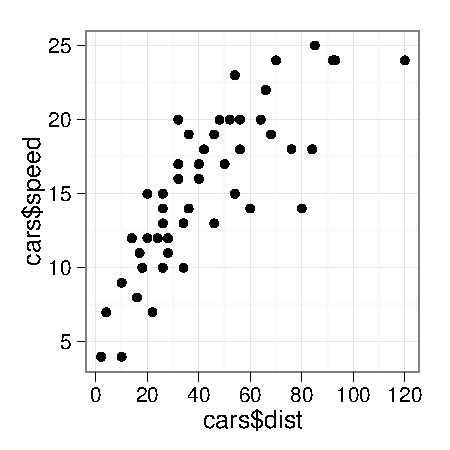
\includegraphics[width=\maxwidth]{images8/Ch8SourceURLExample} 

}


\end{knitrout}


\section{Saving output objects for future use}

\section{Literate Programming: Including highlighted syntax in the output}

\subsection{\LaTeX}

\subsection{Markdown/HTML}

\section{Debugging}

% Chapter Chapter 9 For Reproducible Research in R and RStudio
% Christopher Gandrud
% Created: 16/07/2012 05:45:03 pm CEST
% Updated: 




\chapter{Showing Results with Tables}\ref{TablesChapter}

Graphs and other visual methods, discussed in the next chapter, can
often be a more effective way to present results than tables.\footnote{This
  is especially true of the small-print, high-density coefficient
  estimate tables that are sometimes descriptively called `train
  schedule' tables.} Nonetheless, tables of results, descriptive statistics,
and so on can sometimes be an important part of communicating
research findings.

Creating tables by hand can be tedious no matter what program you are
using to type up your results. Even more tedious is making changes to
hand-created tables when you make changes to your data and models.
Creating these tables can actually introduce new
errors--post-analysis!--if you incorrectly copy what is in your
R output. This is a very real possibility. The mind can go numb
doing that sort of work. Also, creating tables by hand is not very
reproducible.

Fortunately, we don't actually need to create tables by hand. There are
many ways to have R do the work for us. The goal of this
chapter is to learn how to how to \textbf{automate table creation} for
documents produced with both \LaTeX and Markdown/HTML. There are a
number of ways to turn R objects into tables written in
\LaTeX or HTML markup. In this chapter I mostly focus on the
\texttt{xtable} and \texttt{texreg} packages. \texttt{xtable} can
created tables for both of these markup languages. \texttt{texreg} only
produces output for \LaTeX. \texttt{knitr} allows us to incorporate
these tables directly into our documents.

\textbf{Warning:} Automating table creation removes the possibility of
adding errors to our analyses by incorrectly copying R output,
which is a big potential problem in hand-created tables. Be warned, it
is not an error free process. We could easily create inaccurate tables
through coding errors. For example, we may incorrectly merge together
columns in so that our id variables no longer match the data they are
supposed to.

So, as always, it is important to `eyeball' the output. Does it make
sense? If we picked a couple values in the R output do the
match what is in our final table? If not, we need to go back to the code
and see where things have gone wrong. With that caveat, lets start
making tables.

\section{Table Basics}

Before getting into the details of how to create tables from R objects we need to first learn how generic tables are created in \LaTeX and Markdown/HTML.

\subsection{Tables in \LaTeX}

\subsection{Tables in Markdown/HTML}

\section{Creating tables from R objects}

\subsection{\texttt{xtable} \& \texttt{texreg} basics with supported
class objects}

\subsubsection{\texttt{xtable} for \LaTeX}

\subsubsection{\texttt{xtable} for Markdown}

\subsection{\texttt{xtable} with non-supported class objects}

{\tt{xtable}} and other commands in similar packages are very convenient for making tables from objects in supported classes.\footnote{To see a full list of classes that {\tt{xtable}} supports type {\tt{methods(xtable)}} into the R console.} With supported class objects {\tt{xtable}} knows where to look for the vectors containing the things--coefficient names, standard errors, and so on--that it needs to create the table. With unsupported classes, however, it doesn't know where to look for these things. We need to help it out. 

{\tt{xtable}} does have a way of dealing with {\tt{matrix}} and {\tt{dataframe}} class objects. The rows of these objects become the rows of the table and the columns become the table columns. So, to create tables with non-supported class objects we need to

\begin{enumerate}
    \item find and extract the information from the unsupported class object that we want in the table, 
    \item convert this information into a matrix or dataframe where the rows and columns of the object correspond to the rows and columns of the table that we want,
    \item use {\tt{xtable}} with this object to create the table.
\end{enumerate}

Imagine that we want to create a results table showing the covariate names, coefficient means, and quantiles for marginal posterior distributions from a Bayesian normal linear regression using the {\tt{zelig}} command \cite{Goodrich2007} and data from the {\emph{swiss}} dataframe.\footnote{This dataframe is loaded by default.} We run our model:

\begin{knitrout}
\definecolor{shadecolor}{rgb}{0.969, 0.969, 0.969}\color{fgcolor}\begin{kframe}
\begin{alltt}
\hlcomment{# Load required library}
\hlfunctioncall{library}(Zelig)

\hlcomment{# Run model}
NBModel <- \hlfunctioncall{zelig}(Examination ~ Education, model = \hlstring{"normal.bayes"}, 
                    data = swiss, cite = FALSE)

\hlcomment{# Find NBModel's class}
\hlfunctioncall{class}(NBModel)
\end{alltt}
\begin{verbatim}
## [1] "MCMCZelig"
\end{verbatim}
\end{kframe}
\end{knitrout}


Using the {\tt{class}} command we found that the model output object is an {\tt{MCMCZelig}} class object. This class is not supported by {\tt{xtable}}. If we try to create a summary table called {\emph{NBTable}} of the results we will get the following error:

\begin{knitrout}
\definecolor{shadecolor}{rgb}{0.969, 0.969, 0.969}\color{fgcolor}\begin{kframe}


{\ttfamily\noindent\bfseries\textcolor{errorcolor}{\#\# Error: no applicable method for 'xtable' applied to an object of class "MCMCZelig"}}\end{kframe}
\end{knitrout}


With unsupported class objects we have to create the summary ourselves and extract the things that we want from it manually. This is where a good knowledge of vectors comes in handy. 

First, let's create a summary of our output object {\emph{NBModel}}:

\begin{knitrout}
\definecolor{shadecolor}{rgb}{0.969, 0.969, 0.969}\color{fgcolor}\begin{kframe}
\begin{alltt}
NBModelSum <- \hlfunctioncall{summary}(NBModel)
\end{alltt}
\end{kframe}
\end{knitrout}


We created a new object of the class {\tt{summary.MCMCZelig}}. We're still not there yet as this object contains not just the covariate names and so on but also information we don't want to include in our results table like the formula that we used. The second step is to extract a matrix from inside {\emph{NBModelSum}} called {\emph{summary}} with the component selector ({\tt{\$}}). This matrix is where the things we want in our table are located. I find it easier to work with dataframes, so we'll also convert the matrix into a dataframe.

\begin{knitrout}
\definecolor{shadecolor}{rgb}{0.969, 0.969, 0.969}\color{fgcolor}\begin{kframe}
\begin{alltt}
NBSumDataFrame <- \hlfunctioncall{data.frame}(NBModelSum$summary)
\end{alltt}
\end{kframe}
\end{knitrout}

%%
\noindent Here is what our model results dataframe looks like:

\begin{knitrout}
\definecolor{shadecolor}{rgb}{0.969, 0.969, 0.969}\color{fgcolor}\begin{kframe}
\begin{verbatim}
##                Mean      SD   X2.5.    X50.  X97.5.
## (Intercept) 10.1397 1.31673  7.5579 10.1566 12.7058
## Education    0.5786 0.09118  0.3963  0.5781  0.7609
## sigma2      34.9703 7.81260 22.9567 33.8782 53.2172
\end{verbatim}
\end{kframe}
\end{knitrout}


\noindent Now we have a dataframe object that {\tt{xtable}} can handle. After a little cleaning up (see the chapter's source code for more details) we can use {\emph{NBSumDataFrame}} with {\tt{xtable}} as before to create the following table:
\vspace{0.5cm}


% latex table generated in R 2.15.1 by xtable 1.7-0 package
% Mon Sep  3 14:27:22 2012
\begin{table}[ht]
\begin{center}
\begin{tabular}{rrrrr}
  \hline
 & Mean & 2.5\% & 50\% & 97.5\% \\ 
  \hline
(Intercept) & 10.14 & 7.56 & 10.16 & 12.71 \\ 
  Education & 0.58 & 0.40 & 0.58 & 0.76 \\ 
  sigma2 & 34.97 & 22.96 & 33.88 & 53.22 \\ 
   \hline
\end{tabular}
\caption{Coefficient Estimates Predicting Examination Scores in Swiss Cantons (1888) Found Using Bayesian Normal Linear Regression}
\end{center}
\end{table}




It may take a bit of hunting to find what you want, but a similar process can be used to create tables from objects of virtually any class.\footnote{This process can also be used to create graphics.} Hunting for what you want is generally easier by clicking on the object in RStudio's workspace pane.

\subsection{Basic \texttt{knitr} syntax for tables}

So far we have only looked at how to create \LaTeX and HTML tables from R objects. How can we knit these tables into our presentation documents?

The most important \texttt{knitr} chunk option for showing the markup created by these packages as tables is \texttt{results}. The \texttt{results} option can have three values:

\begin{itemize}
\item
  \texttt{markup},
\item
  \texttt{asis},
\item
  \texttt{hide}.
\end{itemize}
\texttt{hide} clearly hides the results of whatever we have in our code chunk; no results show up.

\section{Tables with \texttt{apsrtable}}


% Chapter Chapter 10 For Reproducible Research in R and RStudio
% Christopher Gandrud
% Created: 16/07/2012 05:45:03 pm CEST
% Updated: 2 September 2012




\chapter{Showing Results with Figures}


\section{Basic knitr figure options}

\section{Creating figures with plot and ggplot2}

\section{Animations}

\section{Motion charts and basic maps with GoogleVis}


\part{Presentation Documents}

% Chapter Chapter 11 For Reproducible Research in R and RStudio
% Christopher Gandrud
% Created: 16/07/2012 05:45:03 pm CEST
% Updated: 3 September 2012




\chapter{Presenting with \LaTeX}\ref{LatexChapter}

\section{The Basics}

All commands in \LaTeX start with a \texttt{\textbackslash{}}

\subsection{Editors}

As I mentioned earlier, RStudio is an fully functional \LaTeX editor as well as an integrated development environment for R. Of course it is oriented towards combining R and \LaTeX. If you want to create a new \LaTeX document you can click {\tt{File}} \rightarrow {\tt{New}} \rightarrow {\tt{R\; Sweave}}. 

Remember from Chapter \ref{GettingStarted} that R Sweave\index{R Sweave} files are basically \LaTeX files that can include {\emph{knitr}} code chunks. You can compile R Sweave files like regular \LaTeX files in RStudio even if they do not have code chunks. If you use another program to compile them you might need to change the file extension from {\tt{.Rnw}} to {\tt{.tex}}.

\subsection{The header \& the body}

All \LaTeX documents require a header\index{LaTeX header}. The header goes before the body of the document and specifies what type of presentation document you are creating--an article, a book, a slideshow, and so on. \LaTeX refers to these as classes\index{\LaTeX class}. You also can specify what style it should be formatted in and load any extra packages you may want to use to help you format your document.\footnote{The command to load a package in \LaTeX is \texttt{\textbackslash{}usepackage}. For example, if you include \texttt{\textbackslash{}usepackage\{url\}} in the header of your document you will be able to specify URL links in the body with the command \texttt{\textbackslash{}url\{SOMEURL\}}.}

The header is followed by the body of your document. You tell \LaTeX where the body\index{LaTeX begin document} of your document starts by typing \texttt{\textbackslash{}begin\{document\}}. The very last line of you document is usually \texttt{\textbackslash{}end\{document\}}, indicating that your document has ended. When you open a new R Sweave file in RStudio it creates an article class document with a very simple header and body like this:

\begin{knitrout}
\definecolor{shadecolor}{rgb}{0.969, 0.969, 0.969}\color{fgcolor}\begin{kframe}
\begin{alltt}
\textbackslash{}documentclass\{article\}
\textbackslash{}begin\{document\}
\textbackslash{}end\{document\}
\end{alltt}
\end{kframe}
\end{knitrout}



\subsection{Headings}

\subsection{Footnotes \& Bibliographies}

\subsubsection{Footnotes}

Plain, non-bibliographic footnotes are easy to create in \LaTeX. Simply place \texttt{\textbackslash{}footnote\{} where you would like the footnote number to apear in the text. Then type in the footnote's text and of course remember to close it with a \texttt{\}}. \LaTeX does the rest, including formatting and numbering.

\subsubsection{Bibliographies}

\paragraph{Citing R Packages with BibTeX}

Researchers are pretty good about consistently citing others' articles and data. However, citing the R packages used in an analysis is very inconsistent. This is unfortunate not only because correct attribution is not being given but also because it makes reproducibility harder because it obscures important steps that were taken in the
research process. Fortunately, R actually includes the tools to quickly generate citations, including the version of the package you are using. It can also add them directly to an existing bibliography file.

You can automatically create citations for R packages using the \texttt{citation} command in \emph{base} R. For example if we want the citation information for the \texttt{Zelig} package we would simply type:

\begin{knitrout}
\definecolor{shadecolor}{rgb}{0.969, 0.969, 0.969}\color{fgcolor}\begin{kframe}
\begin{alltt}
\hlfunctioncall{citation}(\hlstring{"ggplot2"})
\end{alltt}
\begin{verbatim}
## 
## To cite ggplot2 in publications, please use:
## 
##   H. Wickham. ggplot2: elegant graphics for data
##   analysis. Springer New York, 2009.
## 
## A BibTeX entry for LaTeX users is
## 
##   @Book{,
##     author = {Hadley Wickham},
##     title = {ggplot2: elegant graphics for data analysis},
##     publisher = {Springer New York},
##     year = {2009},
##     isbn = {978-0-387-98140-6},
##     url = {http://had.co.nz/ggplot2/book},
##   }
\end{verbatim}
\end{kframe}
\end{knitrout}


\noindent This gives us both the plain citation as well as the BibTeX version for use in \LaTeX and MultiMarkdown documents. If you only want the BibTeX version of the citation we can use the \texttt{toBibtex} command in the \emph{utils} package.

\begin{knitrout}
\definecolor{shadecolor}{rgb}{0.969, 0.969, 0.969}\color{fgcolor}\begin{kframe}
\begin{alltt}
\hlfunctioncall{toBibtex}(\hlfunctioncall{citation}(\hlstring{"ggplot2"}))
\end{alltt}
\begin{verbatim}
## @Book{,
##   author = {Hadley Wickham},
##   title = {ggplot2: elegant graphics for data analysis},
##   publisher = {Springer New York},
##   year = {2009},
##   isbn = {978-0-387-98140-6},
##   url = {http://had.co.nz/ggplot2/book},
## }
\end{verbatim}
\end{kframe}
\end{knitrout}


\noindent You can append the citation to your existing BibTeX file using the \texttt{sink} command in \emph{base} R. This command diverts our output and/or the messages to a file. For example, imagine that our existing BibTeX file is called \texttt{biblio.bib}. To add the \emph{Zelig} package citation:

\begin{knitrout}
\definecolor{shadecolor}{rgb}{0.969, 0.969, 0.969}\color{fgcolor}\begin{kframe}
\begin{alltt}
\hlcomment{# Divert output to biblio.bib}
\hlfunctioncall{sink}(file = \hlstring{"biblio.bib"}, 
     append = TRUE, type = \hlfunctioncall{c}(\hlstring{"output"})
     )      
\hlfunctioncall{toBibtex}(\hlfunctioncall{citation}(\hlstring{"ggplot2"})) 
\hlfunctioncall{sink}()
\end{alltt}
\end{kframe}
\end{knitrout}


\noindent This places the citation at the end of our \texttt{biblio.bib} file. It is very important to include the argument \texttt{append = TRUE}. If you don't you will erase the existing file. The argument \texttt{type = c("output")} tells R to include only the output, not the messages.

An even faster way to add citations to a bibliography is with \texttt{write.bibtex} command in the \emph{knitcitations} package. To add the \emph{Zelig} citation to our \texttt{biblio.bib} file we only need to enter:

\begin{knitrout}
\definecolor{shadecolor}{rgb}{0.969, 0.969, 0.969}\color{fgcolor}\begin{kframe}
\begin{alltt}
\hlcomment{# Load package}
\hlfunctioncall{library}(knitcitations)
 
\hlcomment{# Write Zelig citation and}
\hlcomment{# to biblio.bib}
\hlfunctioncall{write.bibtex}(entry = \hlfunctioncall{c}(\hlstring{"ggplot2"}), 
              file = \hlstring{"bibliography.bib"}, append = TRUE)
\end{alltt}
\end{kframe}
\end{knitrout}


\section{Presentations with Beamer}

You can make slideshow presentations with \LaTeX. FILL IN WITH INTRO

{\emph{knitr}} largely the works the same way in in \LaTeX slideshows as it does in article or book class documents. There are a few differences to look out for. 

\paragraph{Slide frames}

A quick way to create each Beamer slide is to use the \texttt{frame} command:

\begin{knitrout}
\definecolor{shadecolor}{rgb}{0.969, 0.969, 0.969}\color{fgcolor}\begin{kframe}
\begin{alltt}
\textbackslash{}frame\{
\}
\end{alltt}
\end{kframe}
\end{knitrout}


\noindent If you want to include highlighted {\emph{knitr}} code chunks on your slides you should add the \texttt{fragile} option to the \texttt{frame} command.\footnote{For a detailed discussion of why you need to use the \texttt{fragile} option with the verbatim environment that {\emph{knitr}} uses to display highlighted text in \LaTeX documents see this blog post by Pieter Belmans: \url{http://pbelmans.wordpress.com/2011/02/20/why-latex-beamer-needs-fragile-when-using-verbatim/}.} Here is an example:

\begin{knitrout}
\definecolor{shadecolor}{rgb}{0.969, 0.969, 0.969}\color{fgcolor}\begin{kframe}
\begin{alltt}
\textbackslash{}begin\{frame\}[fragile]
    An example fragile frame.
\textbackslash{}end\{frame\}
\end{alltt}
\end{kframe}
\end{knitrout}


\paragraph{Results}

By default {\emph{knitr}} hides the results or a code chunk. If you want to show the results in your slideshow simply set the {\tt{results}} option to {\tt{'asis'}}.
% Chapter Chapter 12 For Reproducible Research in R and RStudio
% Christopher Gandrud
% Created: 16/07/2012 05:45:03 pm CEST
% Updated: 27 August 2012




\chapter{Large \LaTeX Documents: Theses, Books, \& Batch Reports}\label{LargeDocs}

In the previous chapter we learned the basics of how to create \LaTeX documents to present our research findings. So far we have only covered basic short documents, like articles. For longer and more complex documents like books we can take advantage of \LaTeX and {\emph{knitr}} options that allow us to separate our files into manageable pieces. The pieces are usually called \index{child files}, which are combined using a \index{parent document}.

These methods can also be used in the creation of \index{batch reports}: documents that present results for a selected part of a data set. For example, a researcher may want create individual reports of answers to survey questions from interviewees with a specific age. In this chapter we will rely on {\emph{knitr}} and shell scripts to create batch reports. 

\section{Planning large documents}

Before discussing the specifics of each of these methods, it's worth taking some time to carefully plan the structure of our child and parent documents.

\subsection{Planning theses and books}

Books and theses have a natural parent-child structure, i.e. they are single documents comprise of multiple chapters. They often include other child-like features such as title pages, bibliographies, figures, and appendices. We could include most of these features directly into one markup file. Clearly this file would become very large and unwieldy. It would be difficult to find one part or section to edit. If of your presentation markup are are difficult to find, they are difficult to reproduce.  

\subsection{Planning batch reports}

COMPLETE

\section{Combining Chapters}

We will cover three methods for including child documents into our parent documents. The first is very simple and uses the \LaTeX command \index{{\tt{\\input}}}. The second using {\emph{knitr}} is slightly more complex, but gives us much more flexibility. The final method is a special case of {\tt{\\input}} that uses the command line program \index{Pandoc} to convert and include child documents written in non-\LaTeX markup languages. 

\subsection{Parent documents}

\paragraph{knitr global options}
{\emph{knitr}} global chunk options\index{global chunk options} and package options\index{package options} should be set at the beginning of the parent document if you want them to apply to the entire presentation document. 

\subsection{Child documents}

\paragraph{Child documents in the same markup language}

\paragraph{Child documents in a different markup language}

You can use the \index{Pandoc} command line program and to convert child documents that are in a different markup language into the primary markup language you are using for your document. If you have Pandoc installed on your computer,\footnote{Pandoc installation instructions can be found at: \url{http://johnmacfarlane.net/pandoc/installing.html}.} you can call it directly from your parent document with R's {\tt{system}} command. 

For example, the \ref{StylisticConventions} part of this book is written in Markdown. The file is called {\emph{StylisticConventions.md}} It was simply faster to write the list of conventions using the simpler Markdown syntax than \LaTeX, which as we saw has a more complicated way of creating lists. However, I want to include this list in my \LaTeX produced book. Pandoc can convert the Markdown document into a \LaTeX file. This file can then be input into my main document with the \LaTeX command {\tt{\\input}}.

Imagine that my parent and {\emph{StylisticConventions.md}} documents are in the same directory. In the parent document I add a code chunk with the options {\tt{echo=FALSE}} and {\tt{results=`hide'}}. In this code chunk I add the following command to convert the Markdown syntax in {\emph{StylisticConventions.md}} to \LaTeX and save it in a file called {\emph{StyleTemp.tex}}.

\begin{knitrout}
\definecolor{shadecolor}{rgb}{0.969, 0.969, 0.969}\color{fgcolor}\begin{kframe}
\begin{alltt}
\hlfunctioncall{system}("pandoc StylisticConventions.md
        -f markdown -t latex -o StyleTemp.tex")
\end{alltt}
\end{kframe}
\end{knitrout}


\noindent The options {\tt{-f markdown}} and {\tt{-t latex}} tell Pandoc to convert {\emph{StylisticConventions.md}} from Markdown to \LaTeX syntax. {\tt{-o StyleTemp.tex}} instructs Pandoc to save the resulting \LaTeX markup to a new file called {\emph{StyleTemp.tex}}. 

After this code chunk we need to tell our parent document to include the converted text. To do this we follow the code chunk with the {\tt{\\input}} command like this:

\begin{knitrout}
\definecolor{shadecolor}{rgb}{0.969, 0.969, 0.969}\color{fgcolor}\begin{kframe}
\begin{alltt}
\textbackslash{}input\{StyleTemp.tex\}
\end{alltt}
\end{kframe}
\end{knitrout}


\noindent Note that using this method to include a child document that needs to be knit will require extra steps not covered in this book.


\section{Creating Batch Reports}

\subsection{stich}
% Chapter Chapter 13 For Reproducible Research in R and RStudio
% Christopher Gandrud
% Created: 16/07/2012 05:45:03 pm CEST
% Updated: 




\chapter{Presenting on the Web and Beyond with Markdown/HTML}

\section{The Basics}

\subsection{Headings}

Headings in Markdown are extremely simple. To create a line in the style
of the topmost heading--maybe a title--just place one hash mark
(\texttt{\#}) at the beginning of the line. The second tier heading just
gets two hashes (\texttt{\#\#}) and so on. You can also put the hash
mark(s) at the end of the heading, but this is not necessary.

\subsection{Footnotes and bibliographies with MultiMarkdown}

\subsection{Math}

\subsection{Drawing figures with CSS}

\section{Simple webpages}

\subsection{RPubs}

\subsection{Hosting webpages with Dropbox}

\section{Presentations with \texttt{Slidify}}

\section{Reproducible websites}

\subsection{Blogging with Tumblr}

\subsection{Jekyll-Bootstrap and GitHub}

see \url{http://jfisher-usgs.github.com/r/2012/07/03/knitr-jekyll/}

\subsection{Jekyll and Github Pages}

\section{Using Markdown for non-HTML output with Pandoc}

Markdown syntax is very simple. So simple, you may be tempted to write many or all of your presentation documents in Markdown. This presents the obvious problem of how to convert your markdown documents to other markup languages if, for example, you would want to create a \LaTeX formatted PDF. 

Pandoc can help solve this problem. Pandoc is a command line program that can convert files written in Markdown, HTML, \LaTeX, and a number of other markup languages\footnote{See the Pandoc website for more details: {\url{http://johnmacfarlane.net/pandoc/}}} to any of the other formats. 

To use Pandoc first install it by following the instructions at {\url{http://johnmacfarlane.net/pandoc/installing.html}}. Luckily you do not need to open a shell window in addition to {\bf{R}} to run Pandoc. Instead you can run all Pandoc commands in {\bf{R}} with the the {\tt{system}} command. 

For example, 

%% Fill In Example with Fake Documents.

  
% Chapter Chapter 14 For Reproducible Research in R and RStudio
% Christopher Gandrud
% Created: 16/07/2012 05:45:03 pm CEST
% Updated: 




\chapter{Chapter 14:}



\bibliographystyle{plain}
\bibliography{/git_repositories/Rep-Res-Book/Source/rep-res-book.bib,/git_repositories/Rep-Res-Book/Source/rep-res-PackagesCited.bib}

\clearpage
\printindex

\end{document}

